% Helper file: compiles the main paper on its own so that supplement.tex can cite its
% table, figure and section numbers (xr package). You do not need to compile it yourself.
% It does not read external references itself, which stops the two documents compiling
% each other in a loop.
\newcommand{\compilemode}{1}
\newcommand{\noexternalrefs}{}
\documentclass{article}

% Formatting
\DeclareUnicodeCharacter{2060}{\nolinebreak} % Prevent unicode (U+2060) error on local complile
\frenchspacing % No double spacing between sentences
\hbadness=1000000 % Turn off \hbox badness warnings
\linespread{1.2} % Set linespace


% Packages
\usepackage[a4paper, left=1.5cm, right=1.5cm, top=2.0cm, bottom=2.0cm]{geometry}
\usepackage{authblk} % For author formatting
\usepackage{caption} % For figure and table captions
\usepackage{cclicenses} % For creative commons license
\usepackage{float} % To force figure location after text
\usepackage{graphicx} % Adds more functionality to graphics for inclusion of figures
%\usepackage{hyperref} % For clickable web links
\usepackage{lscape} % For landscape pages
\usepackage{lineno} % Allows use of \linenumbers to add line numbers 
\usepackage{lmodern} % A scalable font - avoids erros due to non-sclabale fonts
\usepackage{longtable,booktabs}  % For tables
\usepackage{makecell} % For cell formatting in tables
\usepackage{markdown} % allow use of markdown syntax
\usepackage{microtype} % 'Improved' typesetting
\usepackage[nottoc]{tocbibind} % Add references to table of contents
\usepackage{parskip} % Adds white space between paragraphs
\usepackage{pdflscape} % To create landscape pages that show as landscape in PDF viewer
\usepackage{ragged2e} % Better right ragged edges (allows hyphenation)
\usepackage{subcaption} % Allows use of subfigures
\usepackage[super,comma,sort&compress]{natbib} % Citations using superscript
\usepackage{titlesec} % For title spacing
\usepackage[toc,page]{appendix}
\usepackage{url} % Tidy web links
\usepackage[utf8]{inputenc}
\usepackage{verbatim}
\usepackage{xcolor} % For coloured text
\usepackage{xurl} % For url but with more flexible linebreaking
\usepackage{placeins} % to use \FloatBarrier where want a hard break between content (to force and order of text and figures
\usepackage{xr-hyper} % Cross-references between main paper and supplement (see below)
\usepackage[hidelinks]{hyperref}




% Info on wordcounts:
% https://www.overleaf.com/learn/how-to/Is_there_a_way_to_run_a_word_count_that_doesn%27t_include_LaTeX_commands%3F

% To include refs in word count:
%TC:incbib

\newcommand{\detailtexcount}[1]{%
  \immediate\write18{texcount -merge -sum -q #1.tex output.bbl > #1.wcdetail }%
  \verbatiminput{#1.wcdetail}%
}

% Count tables in wordcount (change to 0 0 if tables not included in word count)
%TC:group table 0 1
%TC:group tabular 1 

%%%%%%%% Compile mode %%%%%%%%
% Choose what to compile by setting \compilemode:
%   1 = main paper only (no supplement)
%   2 = supplement only
%   3 = everything (main paper + supplement)
\providecommand{\compilemode}{3} % (supplement.tex and mainpaper.tex set their own mode)

\newif\ifincludemain
\newif\ifincludesupplement
\ifcase\compilemode
  \or \includemaintrue  \includesupplementfalse % 1: main only
  \or \includemainfalse \includesupplementtrue  % 2: supplement only
  \or \includemaintrue  \includesupplementtrue  % 3: everything
  \else \errmessage{compilemode must be 1, 2 or 3}
\fi

% Cross-references between the main paper and the supplement when they are compiled
% as separate PDFs (xr package). In mode 1, numbers of supplementary tables, figures and
% sections are read from supplement.tex; in mode 2 (supplement.tex), numbers of main-paper
% tables and figures are read from mainpaper.tex. latexmkrc compiles these files
% automatically. In mode 3 everything is in one document, so no external files are needed.
\makeatletter
\newcommand*{\addFileDependency}[1]{\typeout{(#1)}\@addtofilelist{#1}\IfFileExists{#1}{}{\typeout{No file #1.}}}
\makeatother
\newcommand*{\myexternaldocument}[1]{\externaldocument{#1}\addFileDependency{#1.tex}\addFileDependency{#1.aux}}
\ifdefined\noexternalrefs\else
  \ifnum\compilemode=1 \myexternaldocument{supplement}\fi
  \ifnum\compilemode=2 \myexternaldocument{mainpaper}\fi
\fi

% Separate reference list for the supplement when everything is compiled together (mode 3).
% The supplement's references are read from supplement.bbl, which latexmk makes by compiling
% supplement.tex (mode 2; see latexmkrc). In the supplement, \suppcitelabels makes citations look
% up, and bibliography items define, labels with the suffix @supp, so supplementary references
% are numbered separately from the main paper's; \suppnoauxcites stops supplement citations
% being written to main.aux, so they are not added to the main paper's reference list.
\makeatletter
\newcommand{\suppcitelabels}{%
  \def\@extra@b@citeb{@supp}%
  \let\supp@orig@lbibitem\@lbibitem
  \def\@lbibitem[##1]##2{\supp@orig@lbibitem[##1]{##2@supp}}%
  \let\supp@orig@bibitem\@bibitem
  \def\@bibitem##1{\supp@orig@bibitem{##1@supp}}%
}
\newcommand{\suppnoauxcites}{%
  \let\supp@orig@cite\cite
  \renewcommand{\cite}[1]{{\@fileswfalse\supp@orig@cite{##1}}}%
}
\makeatother
\ifnum\compilemode=3 \addFileDependency{supplement.tex}\addFileDependency{supplement.aux}\fi

% Abstract: choose length
% Use \shortabstracttrue for the ~300-word abstract,
% or \shortabstractfalse for the ~500-word abstract
\newif\ifshortabstract
\shortabstracttrue

% Alt text for figures (required by ESJ), printed below each caption.
% Use \showalttextfalse to hide it, for example in a preprint.
\newif\ifshowalttext
\showalttextfalse
\newcommand{\alttext}[1]{\ifshowalttext\par\vspace{0.75ex}{\footnotesize\raggedright\textit{Alt text:} #1\par}\fi}

% Number for supplementary material
\newcommand{\beginsupplement}{
    \setcounter{section}{0}
    \renewcommand{\thesection}{S\arabic{section}}
    \setcounter{figure}{0}
    \renewcommand{\thefigure}{S\arabic{figure}}
    \setcounter{table}{0}
    \renewcommand{\thetable}{S\arabic{table}}
    % Unique hyperlink targets, so links to main-paper tables and figures do not jump to the supplement
    \renewcommand{\theHsection}{S\arabic{section}}
    \renewcommand{\theHfigure}{S\arabic{figure}}
    \renewcommand{\theHtable}{S\arabic{table}}
}


\begin{document}

% Ignore title and abstract in word count
%TC:ignore
\title{Thrombolysis and thrombectomy outcomes by stroke severity and timing: a series of emulated target trials using national stroke registry data}


\renewcommand{\thefootnote}{\fnsymbol{footnote}}

% Order to be decided
\author[*1,2]{Michael Allen}
\author[1,2]{Anna Laws}
\author[1,2]{Kerry Pearn}
\author[1,2]{Yinghui Wei}
\author[4]{Peter McMeekin}
\author[3]{Richard Everson}
\author[3]{Mark Kelson}
\author[4]{Jason Scott}
\author[4]{Eleanor Kashouris}
\author[1]{Joao Delgado}
\author[1,2]{Leon Farmer}
\author[1,2]{Lauren Asare}
\author[5]{Ajay Bhalla}
\author[1,2,6]{Martin James}

% Check affiliations - update RDE Name
\affil[1]{\footnotesize University of Exeter Medical School}
\affil[2]{\footnotesize NIHR South West Applied Research Collaboration (ARC)}
\affil[3]{\footnotesize University of Exeter}
\affil[4]{\footnotesize Northumbria University}
\affil[5]{\footnotesize Guy's and St Thomas' NHS Foundation Trust}
\affil[6]{\footnotesize Royal Devon University Healthcare NHS Foundation Trust}
\affil[*]{\footnotesize Corresponding author: m.allen@exeter.ac.uk}

\date{}
\maketitle

\ifincludemain
\section*{Abstract}

\ifshortabstract

\textbf{Background:} Randomised trials have established intravenous thrombolysis (IVT) and mechanical thrombectomy (MT) for ischaemic stroke, but they mostly report 90-day disability and have limited power to describe effects by stroke severity. We estimated effects on several outcomes by stroke severity and treatment strategy using national registry data.

\textbf{Methods:} We used target trial emulation in Sentinel Stroke National Audit Programme (SSNAP) data for patients with ischaemic stroke in England and Wales admitted in 2020--2025. Trials were defined by NIHSS band (1--5, 6--10, 11--15, 16--20, 21--42), treatment (IVT, MT or both), timing (within or after 4.5 hours of onset) and, for late treatment, perfusion imaging. Each treated patient was matched 1:1 to an untreated patient with identical pre-stroke disability, NIHSS band, age band and atrial fibrillation status. Outcomes at discharge were good functional outcome, modified Rankin Scale (mRS), in-hospital death, length of stay and discharge destination, compared using paired tests.

\textbf{Results:} Among 384,334 patients, 56,677 of 56,738 treated patients (99.9\%) were matched across 34 trial groups. Treatment was associated with more good outcomes in 28 groups, lower discharge mRS in 31, fewer deaths in 19 and a different mix of discharge destinations in 27, with more patients going home. Associations were small in mild stroke: with early IVT in NIHSS 1--5 there were 3.0 percentage points more good outcomes and slightly more deaths. The largest associations were with early IVT plus early MT in NIHSS 11--42: 23.3 to 34.2 percentage points more good outcomes and up to 21.3 percentage points fewer deaths. Associations were larger for early than late treatment. Length of stay was usually shorter, by up to 18.6 days.

\textbf{Conclusions:} Reperfusion treatment was associated with better discharge outcomes across most severity and treatment groups, most strongly for early combined treatment in moderate to severe stroke. Residual confounding is possible, so these estimates add detail to, but do not replace, trial evidence.

\else

% TODO: ~500-word abstract (used when \shortabstractfalse is set in main.tex).

\fi

\fi
%TC:endignore

% Footnotes use letters (a, b, c, ...) from the introduction onwards
% (the title page uses symbols for author footnotes)
\renewcommand{\thefootnote}{\alph{footnote}}
\setcounter{footnote}{0}

%%%%%%%% Main paper
\ifincludemain

\newpage

\section{Introduction}

Reperfusion treatment is the main acute treatment for ischaemic stroke. Intravenous thrombolysis (IVT) restores blood flow by dissolving the clot, and mechanical thrombectomy (MT) removes a clot from a large artery using an endovascular device. Both treatments are supported by randomised controlled trials, but those trials were designed to answer whether treatment works in selected patients, not to describe its effect across the full range of patients treated in routine care.

The benefit of IVT was first shown in the NINDS trial of alteplase given within 3 hours of stroke onset\cite{ninds_tissue_1995}. ECASS III extended the treatment window to 4.5 hours\cite{hacke_thrombolysis_2008}. An individual patient data meta-analysis of nine trials then showed that the benefit of alteplase falls as time to treatment increases, and that, within 4.5 hours, treatment improves the chance of a good outcome regardless of age or stroke severity\cite{emberson_effect_2014}. Beyond 4.5 hours, trials have selected patients using advanced brain imaging. In EXTEND, patients with salvageable brain tissue on perfusion imaging benefited from alteplase given 4.5 to 9 hours after onset\cite{ma_thrombolysis_2019}, a finding supported by a pooled analysis of perfusion-selected trials\cite{campbell_extending_2019}. At the mild end of the severity range, the PRISMS trial found no benefit of alteplase over aspirin in patients with minor stroke without disabling deficits, although the trial stopped early\cite{khatri_effect_2018}.

MT was established by a series of trials published in 2015. The HERMES meta-analysis of five of these trials showed that thrombectomy, mostly given with IVT, substantially reduced disability in patients with large-vessel occlusion treated mostly within 6 hours of onset\cite{goyal_endovascular_2016}. The DAWN and DEFUSE 3 trials then showed benefit up to 24 and 16 hours after onset, respectively, in patients selected by clinical--imaging or perfusion mismatch\cite{nogueira_thrombectomy_2018, albers_thrombectomy_2018}. Since then, perfusion imaging has been used increasingly to select patients for late treatment.

These trials provide strong evidence of benefit, but they leave gaps that matter for clinicians, patients and service planners. First, trials report a small number of outcomes, most often the modified Rankin Scale (mRS) at 90 days. Outcomes that matter to patients and health services during the acute admission, such as in-hospital death, length of stay and where patients go after leaving hospital, are rarely reported in detail. Second, trials are powered to detect an overall treatment effect. Subgroup results by stroke severity are therefore imprecise, and some combinations of treatment, timing and severity have little or no trial data. Third, trial populations are selected, for example by age, pre-stroke disability or imaging criteria, and may not represent all patients treated in practice.

Large national stroke registers can help fill these gaps. The Sentinel Stroke National Audit Programme (SSNAP) collects data on more than 90\% of stroke admissions in England and Wales\cite{ssnap_website}. However, simple comparisons of treated and untreated patients in registry data are prone to bias. Target trial emulation addresses this by first specifying the randomised trial that would ideally be run, and then emulating its eligibility criteria, treatment strategies, outcomes and analysis as closely as possible using observational data\cite{hernan_using_2016, hernan_target_2022}.

This study uses target trial emulation in SSNAP data to estimate the effects of IVT and MT in routine practice in more detail than existing trials allow. We emulated a separate trial for each combination of stroke severity (NIHSS 1--5, 6--10, 11--15, 16--20 and 21--42), treatment (IVT alone, MT alone, or both), treatment timing (within or after 4.5 hours of onset) and, for late treatment, use of perfusion imaging. For each trial we report five outcomes at discharge from hospital: good functional outcome, in-hospital death, disability (mRS), length of stay and discharge destination. We address three questions: how the association between treatment and outcome varies with stroke severity; how it varies with the type and timing of treatment; and whether the pattern is consistent across outcomes.

\section{Methods}

We emulated a series of target trials of reperfusion treatment using national stroke registry data. Each trial compared patients who received one treatment strategy with matched patients who received no reperfusion treatment.

\subsection{Data source and access}

We used anonymised data from the Sentinel Stroke National Audit Programme (SSNAP), the national stroke registry for England and Wales, for stroke admissions in the six calendar years 2020--2025 inclusive\cite{ssnap_website}. Data access was managed through the Healthcare Quality Improvement Partnership (HQIP; \url{https://www.hqip.org.uk/}, Data Request HQIP515). SSNAP collects a core dataset on the care of patients admitted to hospital with stroke, from arrival to discharge.

Before analysis, records were excluded if stroke type was not recorded, if any item of the arrival National Institutes of Health Stroke Scale (NIHSS)\cite{brott_measurements_1989} was missing, or if any recorded time interval (onset to arrival, arrival to brain imaging, arrival to thrombolysis, or arrival to thrombectomy) was negative. Onset-to-arrival times were set to missing when the time of stroke onset was not known. Where the indicators of in-hospital death disagreed (death date, stroke unit death, discharge modified Rankin Scale (mRS) of 6 and discharge destination of `died'), all death-related outcomes for that patient were set to missing. Age is recorded in SSNAP in 5-year bands (under 40, 40--44, \ldots, 85--89, 90 and over), and each patient was assigned the midpoint of their band.

\subsection{Study population}

The analysis included patients with ischaemic stroke (infarction) who had a recorded mRS at discharge\cite{van_swieten_interobserver_1988}. Patients recorded as receiving intravenous thrombolysis (IVT) after the start of mechanical thrombectomy (MT) were excluded. Stroke severity was classified from the NIHSS on arrival into five bands: 1--5, 6--10, 11--15, 16--20 and 21--42. Patients with an arrival NIHSS of 0 fell outside these bands and were not eligible for any trial.

\subsection{Target trial emulation}

We used target trial emulation\cite{hernan_using_2016, hernan_target_2022}. For each treatment strategy, we specified the randomised trial we would ideally run and then emulated it as closely as possible in the registry data. Table~\ref{tab:target_trial} summarises the protocol of the target trials and how each part was emulated. The TARGET statement guided our reporting\cite{cashin_target_2025}.

\begin{table}[H]
\centering
\small
\caption{Specification of the target trials and their emulation using SSNAP data.}
\label{tab:target_trial}
\begin{tabular}{p{2.8cm} p{6.6cm} p{6.6cm}}
\toprule
\textbf{Component} & \textbf{Target trial} & \textbf{Emulation} \\
\midrule
Eligibility & Adults admitted with ischaemic stroke and an arrival NIHSS within the trial's severity band. & SSNAP patients with infarction, an arrival NIHSS within the band, and a recorded discharge mRS. Patients receiving IVT after MT were excluded. \\
\addlinespace
Treatment strategies & Treatment with the trial's reperfusion strategy (IVT and/or MT, early or late, with or without perfusion imaging for late treatment) versus no reperfusion treatment. & Treated arm: patients in the band whose recorded treatment exactly matched the trial's pattern. Control arm: patients in the band who received neither IVT nor MT. \\
\addlinespace
Assignment & Random allocation. & 1:1 exact matching on pre-stroke mRS, NIHSS band, age band, anticoagulant use for atrial fibrillation (AF), and AF diagnosis. \\
\addlinespace
Time zero & Stroke onset. & Stroke onset. Treatment times were measured from onset, and treatment status was taken from treatment received during the admission. \\
\addlinespace
Follow-up & From stroke onset until discharge or in-hospital death. & From stroke onset until discharge or in-hospital death. \\
\addlinespace
Outcomes & Good functional outcome at discharge; in-hospital death; discharge mRS; length of stay; discharge destination. & As in the target trial, taken from SSNAP discharge data. \\
\addlinespace
Causal contrast & Effect of the treatment strategy compared with no reperfusion treatment. & Effect of treatment in the treated (patients who received the strategy), estimated from matched pairs. \\
\addlinespace
Analysis & Comparison of outcomes between randomised arms. & Paired comparison of outcomes within matched pairs, with Holm adjustment across trial groups. \\
\bottomrule
\end{tabular}
\end{table}

\subsection{Treatment strategies and trial groups}

Treatment times were measured from stroke onset. Treatment was classed as early if it started within 270 minutes (4.5 hours) of onset, the time window within which the benefit of IVT is established\cite{emberson_effect_2014}, and as late otherwise. For IVT this used the onset-to-needle time, and for MT the onset-to-arterial-puncture time. When the time of stroke onset was not known, so that onset-to-treatment time could not be calculated, treatment was classed as late.

Each trial group was defined by a stroke severity band, a combination of early and/or late IVT and MT, and, for groups that included late treatment, whether perfusion imaging was used. Treated patients had to match the group's treatment pattern exactly. For example, the `IVT early' group included only patients who received early IVT and no MT. In groups with any late treatment, perfusion imaging status also had to match the group definition, so `MT late' means late MT without recorded perfusion imaging. Groups with only early treatment included patients whether or not perfusion imaging was used. Perfusion imaging is recorded in the thrombectomy (intra-arterial intervention) section of the SSNAP dataset.

Thirty-nine trial groups were defined. In the text, figures and tables, groups are named by treatment and timing, with `(perfusion)' marking late treatment with perfusion imaging. In the NIHSS 1--5 and 6--10 bands, three IVT-only groups were defined: IVT early, IVT late, and IVT late (perfusion). MT groups were not defined for these bands. In each of the NIHSS 11--15, 16--20 and 21--42 bands, eleven groups were defined:
\begin{itemize}
    \item IVT only: IVT early; IVT late; IVT late (perfusion).
    \item MT only: MT early; MT late; MT late (perfusion).
    \item IVT and MT: IVT early + MT early; IVT early + MT late; IVT early + MT late (perfusion); IVT late + MT late; IVT late + MT late (perfusion).
\end{itemize}

\subsection{Matching}

For each trial group, the pool of potential controls was all patients in the same NIHSS band who received neither IVT nor MT and who had complete data on the matching variables. Each treated patient was matched 1:1, without replacement, to an untreated patient with identical values of all five matching variables: pre-stroke mRS, NIHSS band, age band, anticoagulant use for AF, and AF diagnosis (pre-existing or newly diagnosed on admission)\cite{stuart_matching_2010}. Within each combination of matching variables, treated and untreated patients were put in random order and paired off. Treated patients left without a match, including those missing any matching variable, were excluded from that trial, and the percentage of treated patients matched was recorded for each group (Supplementary Table~\ref{tab:supp_matching}). Matching was carried out separately for each trial group, so an untreated patient could serve as a control in more than one trial group. A fixed random seed was used for reproducibility.

The matching variables describe the patient before or at admission, and are related to both the likelihood of treatment and outcome. Exact matching was possible because the pool of untreated patients was large.

\subsection{Outcomes}

Five outcomes were assessed at hospital discharge:
\begin{itemize}
    \item \textbf{Good outcome} (binary): discharge mRS of 2 or less, or discharge mRS no worse than pre-stroke mRS. The second condition allows patients who had disability before their stroke to have a good outcome if they return to their previous level.
    \item \textbf{In-hospital death} (binary).
    \item \textbf{Discharge disability}: mRS at discharge (0--6, where 6 is death), analysed as a continuous outcome.
    \item \textbf{Length of stay} (continuous): days from arrival to hospital discharge, or to death for patients who died in hospital.
    \item \textbf{Discharge destination} (categorical): home; community team or early supported discharge; transfer to a hospital team not in SSNAP; care home; somewhere else; or died. Destinations recorded as missing were treated as missing data.
\end{itemize}

\subsection{Statistical analysis}

Each trial group was analysed as a separate emulated trial, comparing treated patients with their matched controls. Because controls were chosen to resemble the treated patients, the comparison estimates the average effect of treatment in the treated: the effect in patients like those who actually received each treatment. For each outcome, pairs in which either patient had a missing outcome were excluded, and missing data were not imputed. All analyses used paired methods.

We described the baseline characteristics of the matched patients in each trial group. For characteristics not used in matching (arrival NIHSS within the band, sex, hypertension, diabetes and congestive heart failure), balance between arms was summarised with the standardised mean difference (SMD): the difference in means between treated and untreated patients divided by the pooled standard deviation. We also described onset-to-treatment times in the treated arm.

For binary outcomes (good outcome and in-hospital death), we report the percentage with the outcome in each arm and the difference in percentage points (treated minus untreated). The 95\% confidence interval (CI) of the difference was calculated from the mean and standard deviation of the within-pair differences using a normal approximation. We also report the matched-pair odds ratio, calculated from discordant pairs as the number of pairs in which only the treated patient had the outcome divided by the number in which only the control had it. Its 95\% CI was calculated on the log scale. The odds ratio was not calculated when there were no discordant pairs in one direction. Differences were tested with McNemar's test\cite{mcnemar_note_1947}, using the exact binomial version when there were fewer than 25 discordant pairs and the continuity-corrected chi-squared version otherwise.

For continuous outcomes (discharge mRS and length of stay), we report the mean, standard deviation, median and interquartile range in each arm, and the mean within-pair difference with a 95\% CI based on the $t$ distribution. Because discharge mRS is ordinal and length of stay is right-skewed, the Wilcoxon signed-rank test\cite{wilcoxon_individual_1945} was the primary test. A paired $t$-test was also calculated and is available with the analysis code.

For discharge destination, we report the percentage of patients in each category in each arm. Marginal homogeneity between arms was tested with the Stuart--Maxwell test\cite{stuart_comparison_1957, maxwell_comparing_1970}.

Because many trial groups were tested for each outcome, $p$-values were adjusted across trial groups within each outcome using the Holm method\cite{holm_simple_1979}. Results with a Holm-adjusted $p$-value below 0.05 were considered statistically significant.

Each trial group has its own matched control group, so each trial estimates the effect of one treatment strategy compared with no reperfusion treatment. We did not formally compare treatment strategies with each other. Differences between trial groups are described but not tested.

\subsection{Software and code availability}

Analyses were carried out in Python 3.12 using pandas\cite{mckinney_data_2010}, NumPy\cite{harris_array_2020}, SciPy\cite{virtanen_scipy_2020}, statsmodels\cite{seabold_statsmodels_2010} and Matplotlib\cite{hunter_matplotlib_2007}. All analysis code is available on GitHub.\footnote{\url{https://github.com/samuel-book/samuel-3/blob/main/4_target_trial_emulation/03_target_trials_all_patients_treatments.ipynb}}

% TODO: Add ethics/approvals statement if required by the journal.

\section{Results}

\subsection{Study population and matching}

Of 452,863 admissions in the cleaned data, 384,334 had an ischaemic stroke with a recorded discharge mRS and did not receive IVT after MT, and 343,739 of these had an arrival NIHSS of 1 to 25 (Supplementary Figure~\ref{fig:supp_flow}). Of the 343,739, 58,074 received IVT and/or MT and 285,665 received neither. Five of the 39 trial groups (IVT late (perfusion)) had no treated patients. In the remaining 34 groups, 54,637 of 54,703 treated patients (99.9\%) were matched to an untreated control, and group sizes ranged from 51 to 13,618 matched pairs (Supplementary Table~\ref{tab:supp_matching}). A further 3,371 treated patients did not fit any trial group (for example, MT in NIHSS 1--10). Outcome data were almost complete: length of stay was missing for 4 treated and 6 untreated patients, and discharge destination for 1 treated and 2 untreated patients.

Mean age ranged from 67.0 to 78.4 years across groups (Supplementary Table~\ref{tab:baseline_matched}). Patients given MT alone often had AF (36\% to 62\%) and were often anticoagulated (23\% to 54\%). Characteristics not used in matching were generally similar between arms, but diabetes was less common in treated patients in 30 of 34 groups, and within NIHSS 1--5 treated patients had higher arrival NIHSS than their controls (mean 3.7 \textit{vs} 2.6 for early IVT; Supplementary Table~\ref{tab:supp_baseline_unmatched}).

\subsection{Outcomes}

After Holm adjustment, treatment was associated with more good outcomes in 27 of 34 groups (Figure~\ref{fig:outcome_target}), fewer in-hospital deaths in 19 and more in 2 (Figure~\ref{fig:death}), lower discharge mRS in 30 (Figure~\ref{fig:discharge_disability}), shorter stays in 14 and longer in none (Figure~\ref{fig:length_of_stay}), and a different mix of discharge destinations in 25, with more patients going home (Figure~\ref{fig:discharge_destination}). Detailed results for each outcome are given in Supplementary Section~\ref{sec:supp_results}.

In mild stroke (NIHSS 1--5), associations were small. Early IVT was associated with 3.0 percentage points (pp) more good outcomes (95\% CI 2.0 to 4.0) and with 0.8 pp (0.5 to 1.1) more in-hospital deaths (2.0\% \textit{vs} 1.2\%). Late IVT was associated with more in-hospital deaths (2.8\% \textit{vs} 1.0\%) and with a small decrease in good outcome that was not statistically significant after adjustment for multiple comparisons ($-$3.1 pp, $-$6.1 to $-$0.1; Holm-adjusted $p = 0.310$).

In moderate to severe stroke (NIHSS 6--25), associations were larger. Early IVT was associated with 16.0 pp (NIHSS 6--10), 19.9 pp (11--15), 17.7 pp (16--20) and 12.8 pp (21--25) more good outcomes, and with reductions in mean discharge mRS of 0.48 to 0.69 points. The largest associations were with early IVT plus early MT: 34.2 pp (NIHSS 11--15), 28.4 pp (16--20) and 25.6 pp (21--25) more good outcomes, reductions in discharge mRS of 1.17 to 1.32 points, stays 18.6 and 18.1 days shorter in NIHSS 11--15 and 16--20, and 20.6 to 31.2 pp more patients discharged home or with community team support. In NIHSS 21--25, in-hospital death was lower by 9.9 pp with early IVT, 18.3 pp with early MT and 18.8 pp with early IVT plus early MT. After late MT in NIHSS 21--25, stays were 3.5 days longer, although this was not statistically significant ($-$1.4 to 8.3), alongside 8.7 pp fewer in-hospital deaths.

\subsection{Patterns across stroke severity, treatment and timing}

These comparisons between trial groups are descriptive, because each group has its own matched controls. Outcomes in untreated controls worsened steeply with severity: good outcome fell from about 75\% in NIHSS 1--5 to between 5\% and 11\% in NIHSS 21--25, and in-hospital death rose from about 1\% to between 31\% and 44\%. With early IVT, the difference in good outcome was largest in NIHSS 11--15, whereas the reduction in in-hospital death grew steadily with severity.

Associations were generally larger for early than for late treatment. For MT alone, the difference in good outcome was 17.1 \textit{vs} 11.5 pp for early \textit{vs} late MT in NIHSS 11--15, 18.8 \textit{vs} 10.6 pp in 16--20 and 19.2 \textit{vs} 9.0 pp in 21--25. Among patients given early IVT and MT, it was 34.2 \textit{vs} 17.1, 28.4 \textit{vs} 17.9 and 25.6 \textit{vs} 13.4 pp when MT was early rather than late. The exception was IVT alone in NIHSS 21--25 (15.7 pp late \textit{vs} 12.8 pp early, from only 217 pairs with late IVT). In every band with MT groups, early IVT plus early MT was associated with larger differences than either treatment alone. For late MT alone, the difference was smaller with perfusion imaging than without in NIHSS 11--15 (3.5 \textit{vs} 11.5 pp) and 21--25 (6.0 \textit{vs} 9.0 pp), and similar in 16--20 (11.8 \textit{vs} 10.6 pp). The groups without a significant difference in good outcome were late IVT in NIHSS 1--5 and six groups with late MT and perfusion imaging, all with fewer than 450 pairs.

\subsection{Sensitivity analyses}

The main findings were robust (Supplementary Section~\ref{sec:supp_sensitivity} and Supplementary Table~\ref{tab:sensitivity}). With matching on exact NIHSS or on more characteristics, with restriction to patients with a known onset time, and after excluding pairs with very early death or discharge, the differences in good outcome and in-hospital death had the same direction as in the primary analysis in at least 32 of 34 groups, with median changes of at most 1.2 pp. Matching on exact NIHSS increased the association with early IVT in NIHSS 1--5 to 9.6 pp more good outcomes (8.6 to 10.7) and halved the excess of in-hospital deaths (0.39 pp, 0.06 to 0.71). Restricting MT groups to patients with a recorded LVO (26\% of treated patients in these groups) gave larger associations, with a median of 6.5 pp more good outcomes and 6.7 pp fewer deaths, in much smaller groups. In pairs in which both patients survived, length of stay was shorter with treatment in 19 groups, compared with 14 in the primary analysis, and the estimate after late MT in NIHSS 21--25 changed from 3.5 days longer to 4.6 days shorter ($-$12.4 to 3.3), although neither difference was statistically significant. E-values were 4.1 to 8.9 for good outcome with early IVT plus early MT, 2.0 to 4.0 for good outcome with early IVT in NIHSS 6--25, and 1.9 to 2.2 for in-hospital death with early IVT in NIHSS 11--25 (Supplementary Table~\ref{tab:supp_evalues}).

% Good outcome

\begin{figure}
\centering
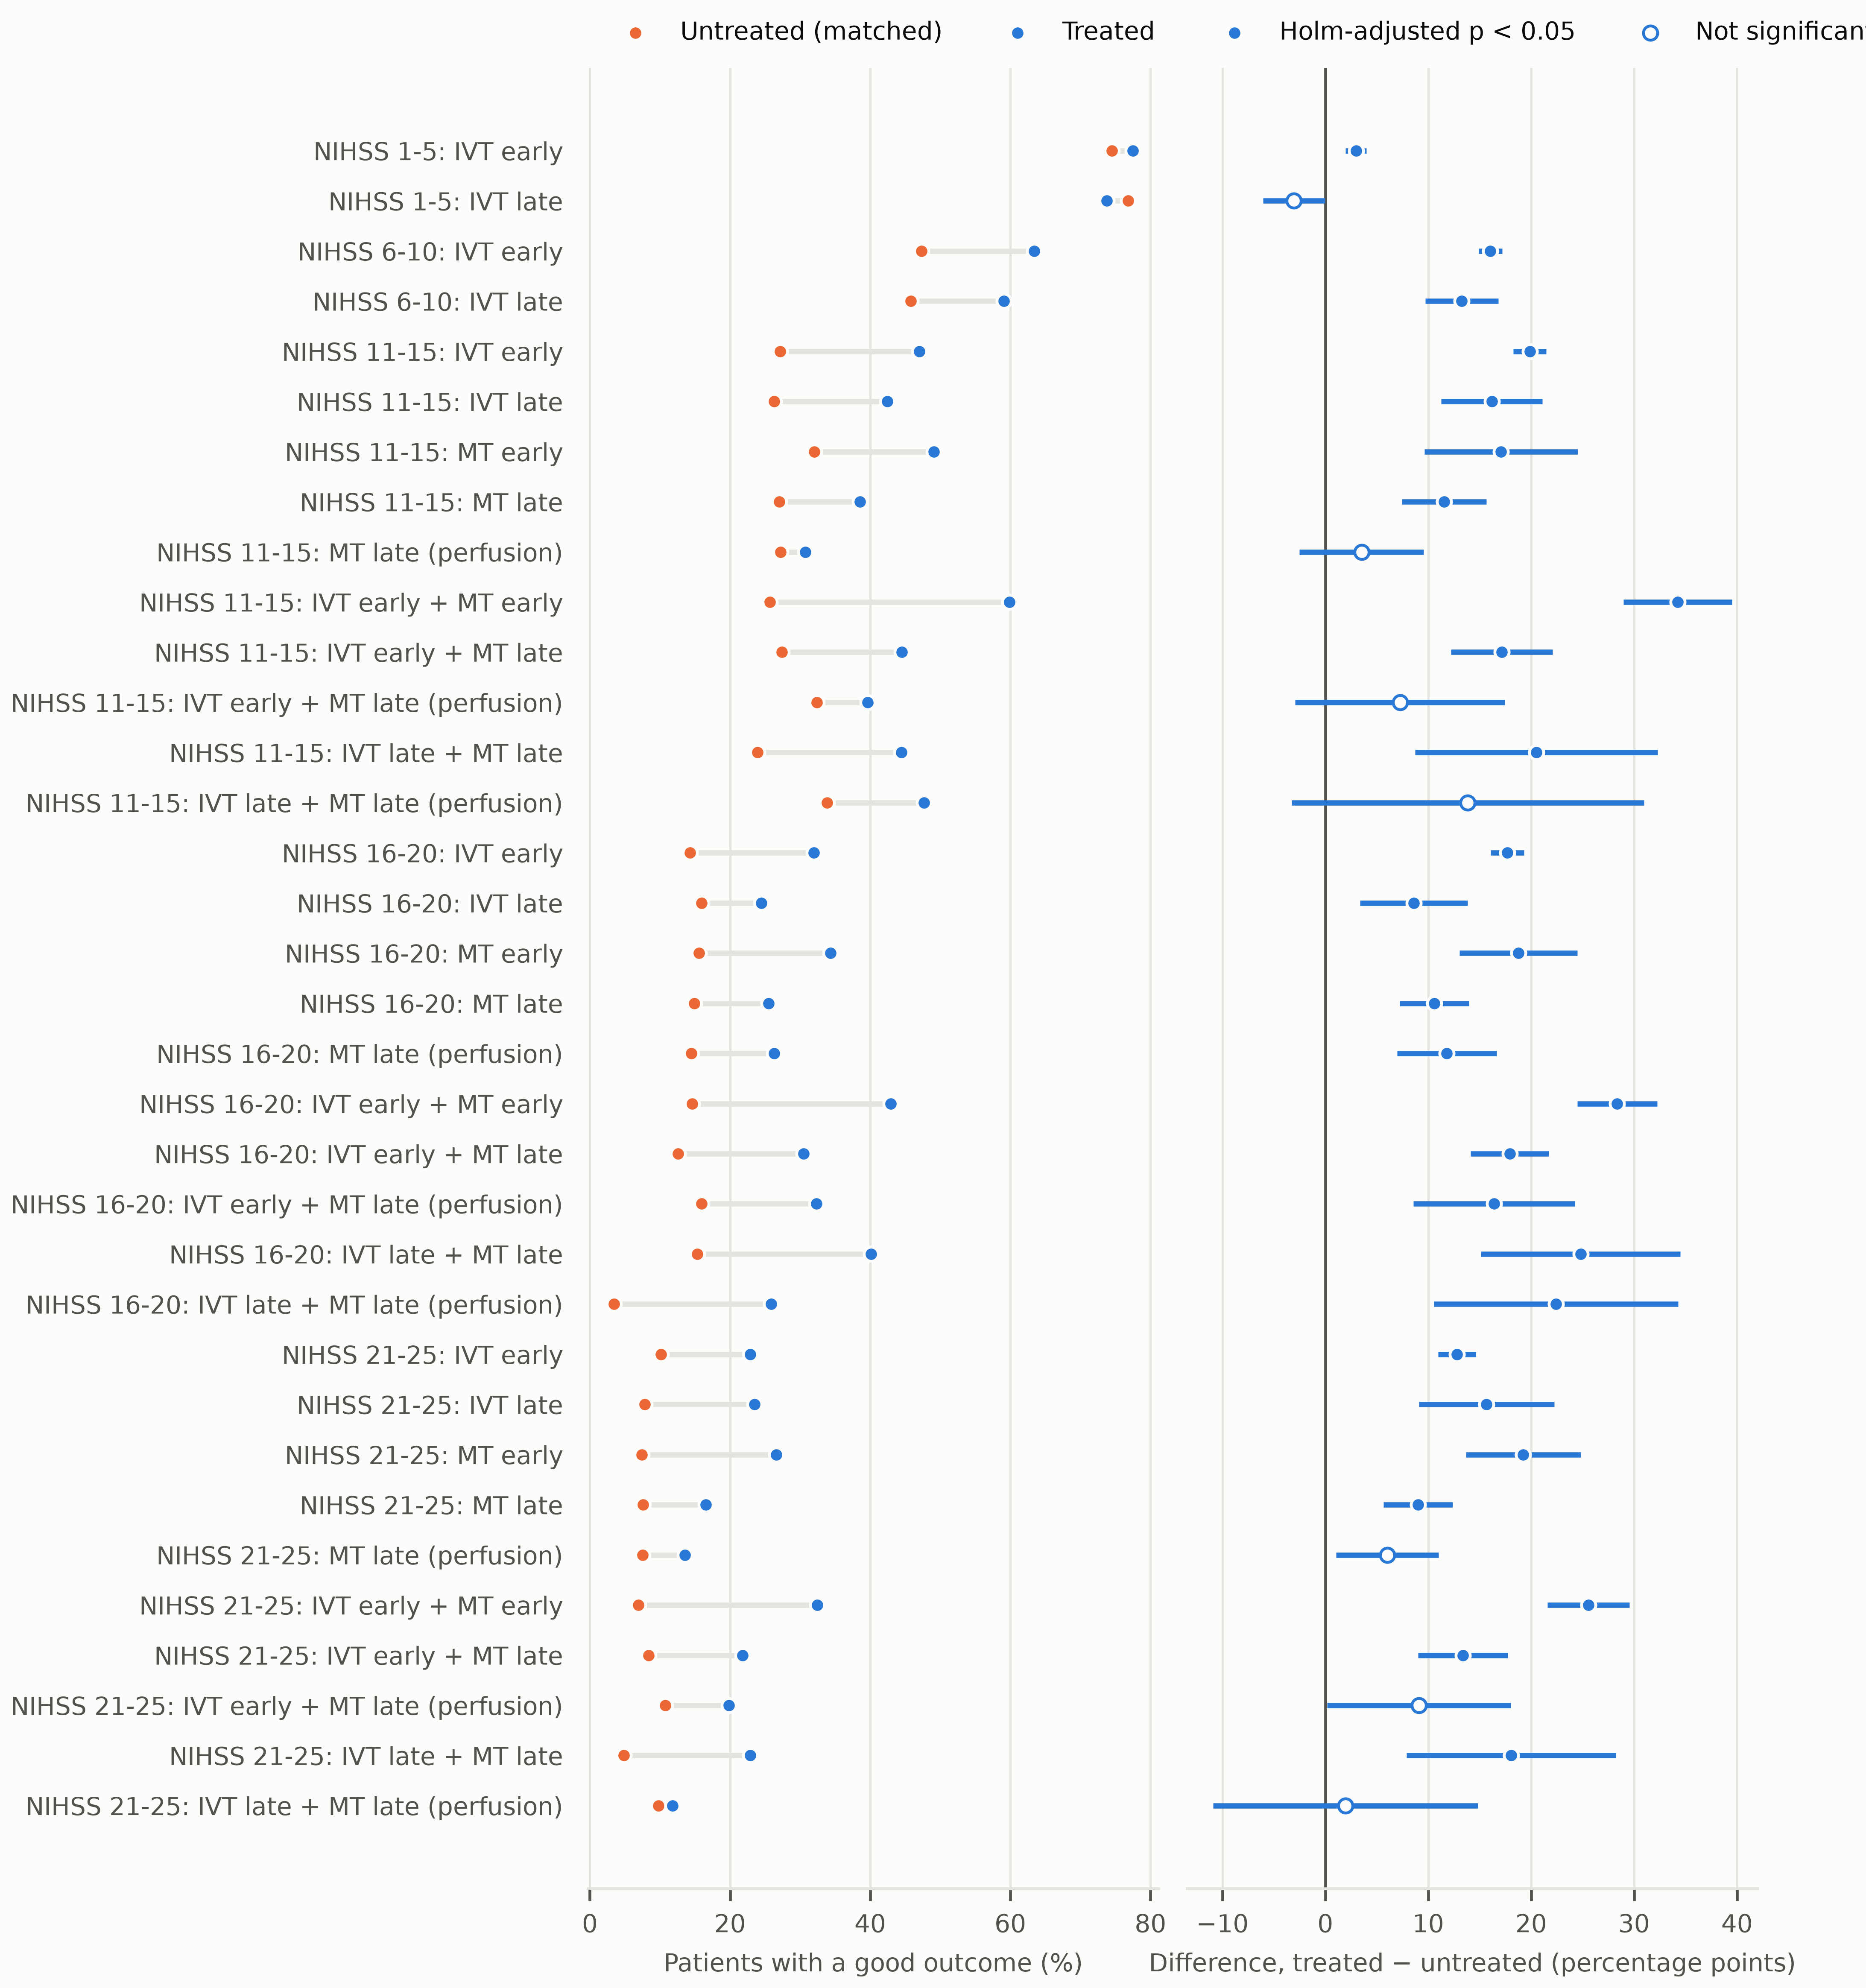
\includegraphics[width=1\linewidth]{chapters/images/all_ischaemic_stroke_target_trials_outcome_target_chart.png}
\caption{Good outcome at discharge (mRS $\le$ 2, or no worse than before the stroke) in each trial group. Left: percentage of treated patients (blue) and matched untreated controls (orange) with a good outcome. Right: difference between arms (treated minus untreated, percentage points) with 95\% confidence interval; filled markers show a Holm-adjusted $p < 0.05$ (McNemar's test). Higher is better. Full results are given in Supplementary Table~\ref{tab:supp_outcome_target}.}
\label{fig:outcome_target}
{\small\textit{Alt text:} Two-panel dot plot for 34 trial groups ordered by stroke severity band. The left panel shows the percentage of treated and matched untreated patients with a good outcome at discharge. The right panel shows the difference in percentage points with 95\% confidence intervals. Most differences are positive, and the largest are for early thrombolysis plus early thrombectomy in moderate to severe stroke.\par}
\end{figure}

% Death

\begin{figure}
\centering
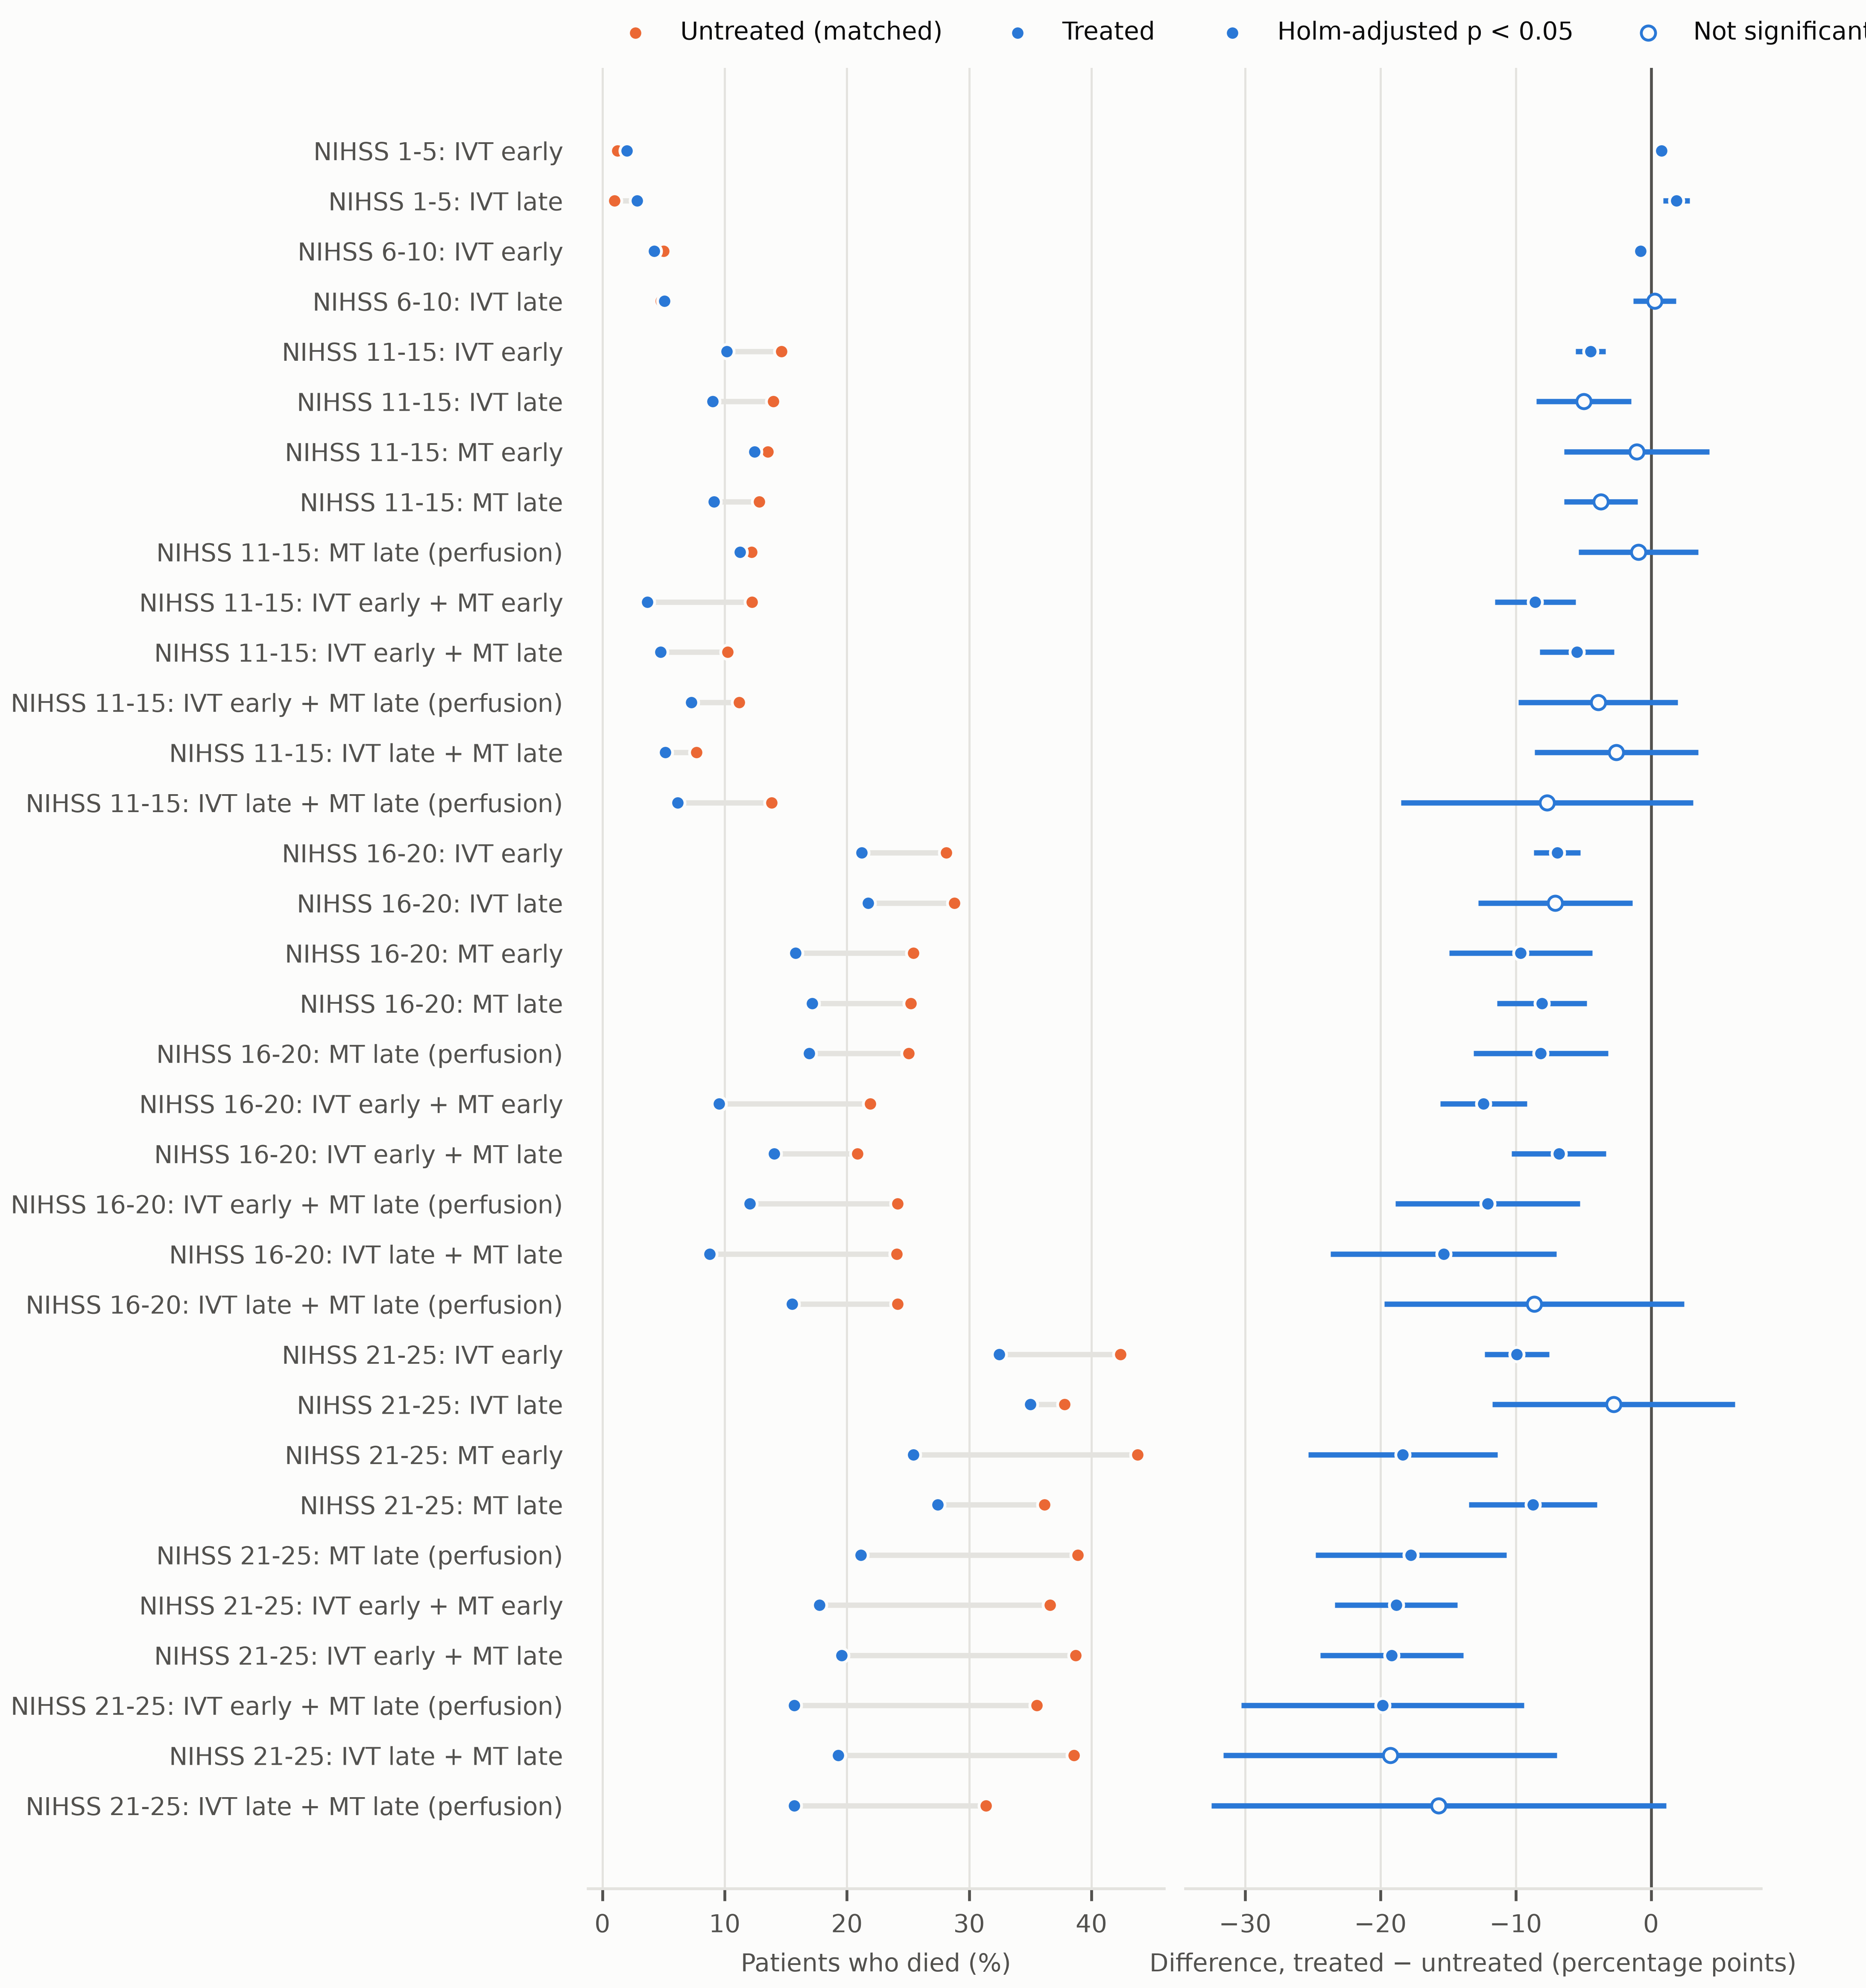
\includegraphics[width=1\linewidth]{chapters/images/all_ischaemic_stroke_target_trials_death_chart.png}
\caption{In-hospital death in each trial group. Left: percentage of treated patients (blue) and matched untreated controls (orange) who died in hospital. Right: difference between arms (treated minus untreated, percentage points) with 95\% confidence interval; filled markers show a Holm-adjusted $p < 0.05$ (McNemar's test). Lower is better. Full results are given in Supplementary Table~\ref{tab:supp_death}.}
\label{fig:death}
{\small\textit{Alt text:} Two-panel dot plot for 34 trial groups ordered by stroke severity band. The left panel shows the percentage of treated and matched untreated patients who died in hospital. The right panel shows the difference in percentage points with 95\% confidence intervals. Deaths are slightly more common with thrombolysis in mild stroke and less common with treatment in most moderate and severe stroke groups.\par}
\end{figure}

% Discharge disability

\begin{figure}
\centering
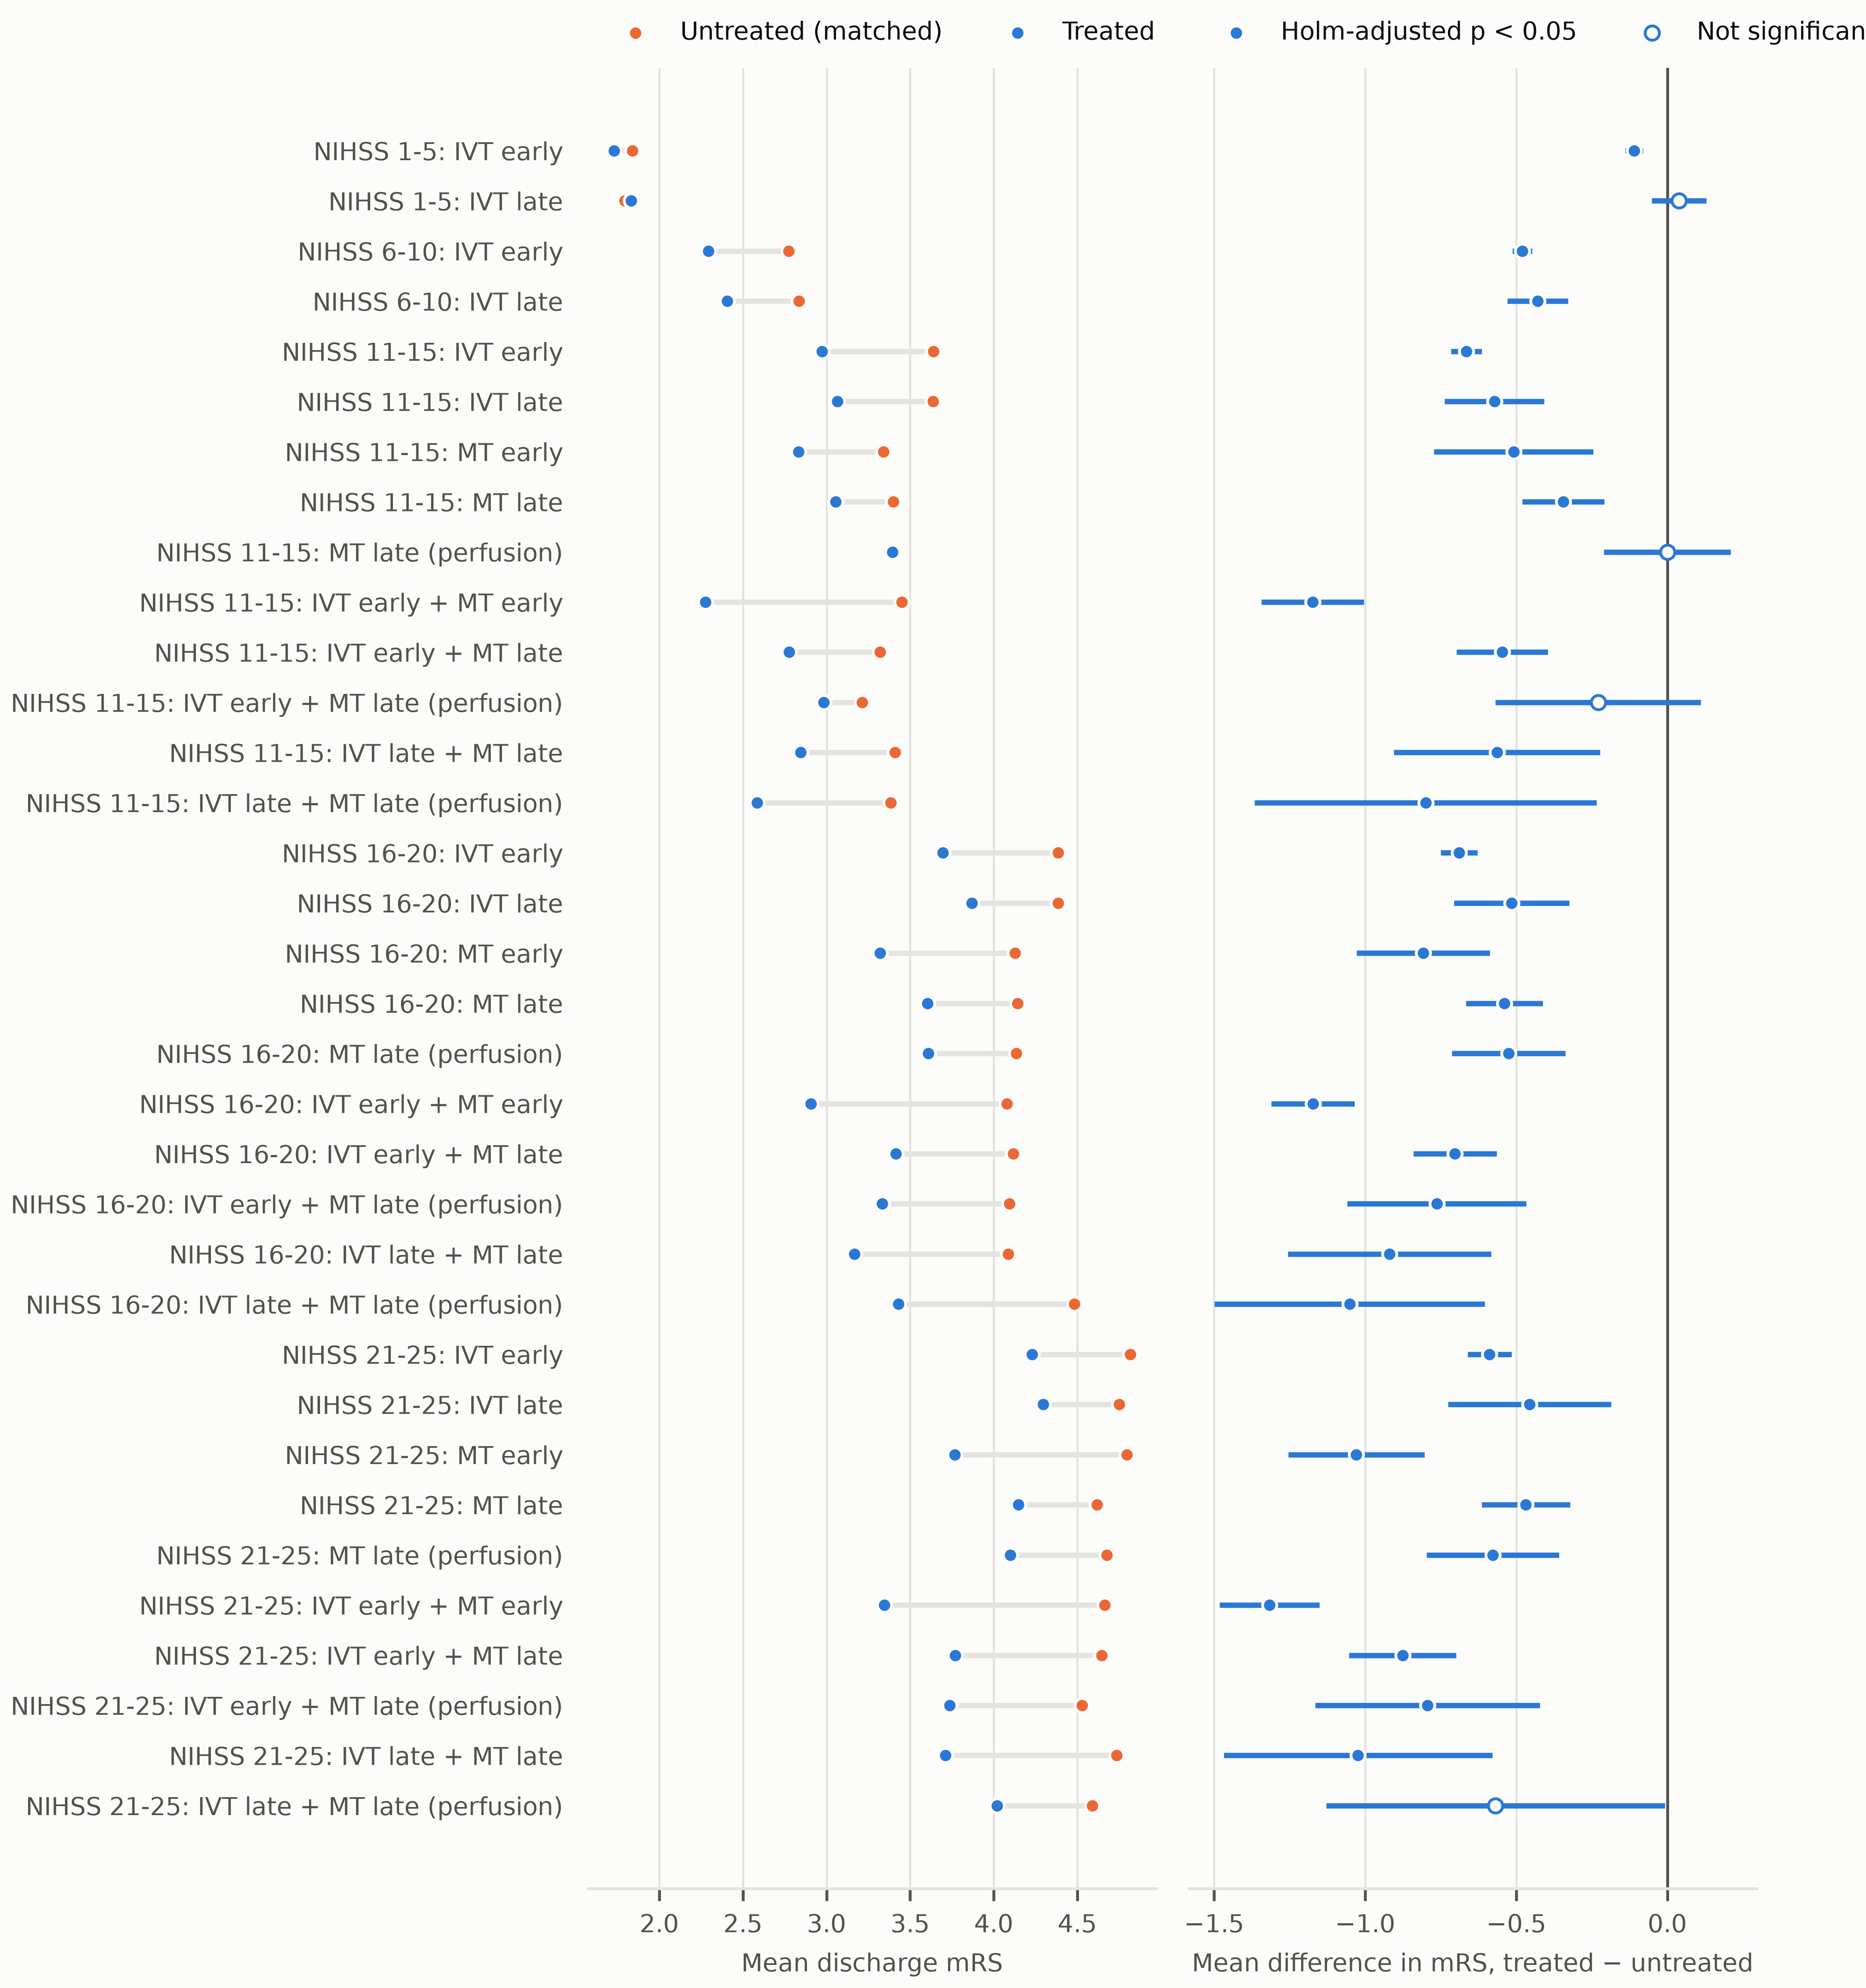
\includegraphics[width=1\linewidth]{chapters/images/all_ischaemic_stroke_target_trials_discharge_disability_chart.png}
\caption{Disability at discharge (modified Rankin Scale, 0--6) in each trial group. Left: mean discharge mRS of treated patients (blue) and matched untreated controls (orange). Right: mean within-pair difference (treated minus untreated) with 95\% confidence interval; filled markers show a Holm-adjusted $p < 0.05$ (Wilcoxon signed-rank test). Lower is better. Full results are given in Supplementary Table~\ref{tab:supp_discharge_disability}.}
\label{fig:discharge_disability}
{\small\textit{Alt text:} Two-panel dot plot for 34 trial groups ordered by stroke severity band. The left panel shows mean modified Rankin Scale score at discharge in treated and matched untreated patients. The right panel shows the mean difference with 95\% confidence intervals. Treated patients have lower scores in most groups, with the largest reductions for early thrombolysis plus early thrombectomy.\par}
\end{figure}

% Length of stay

\begin{figure}
\centering
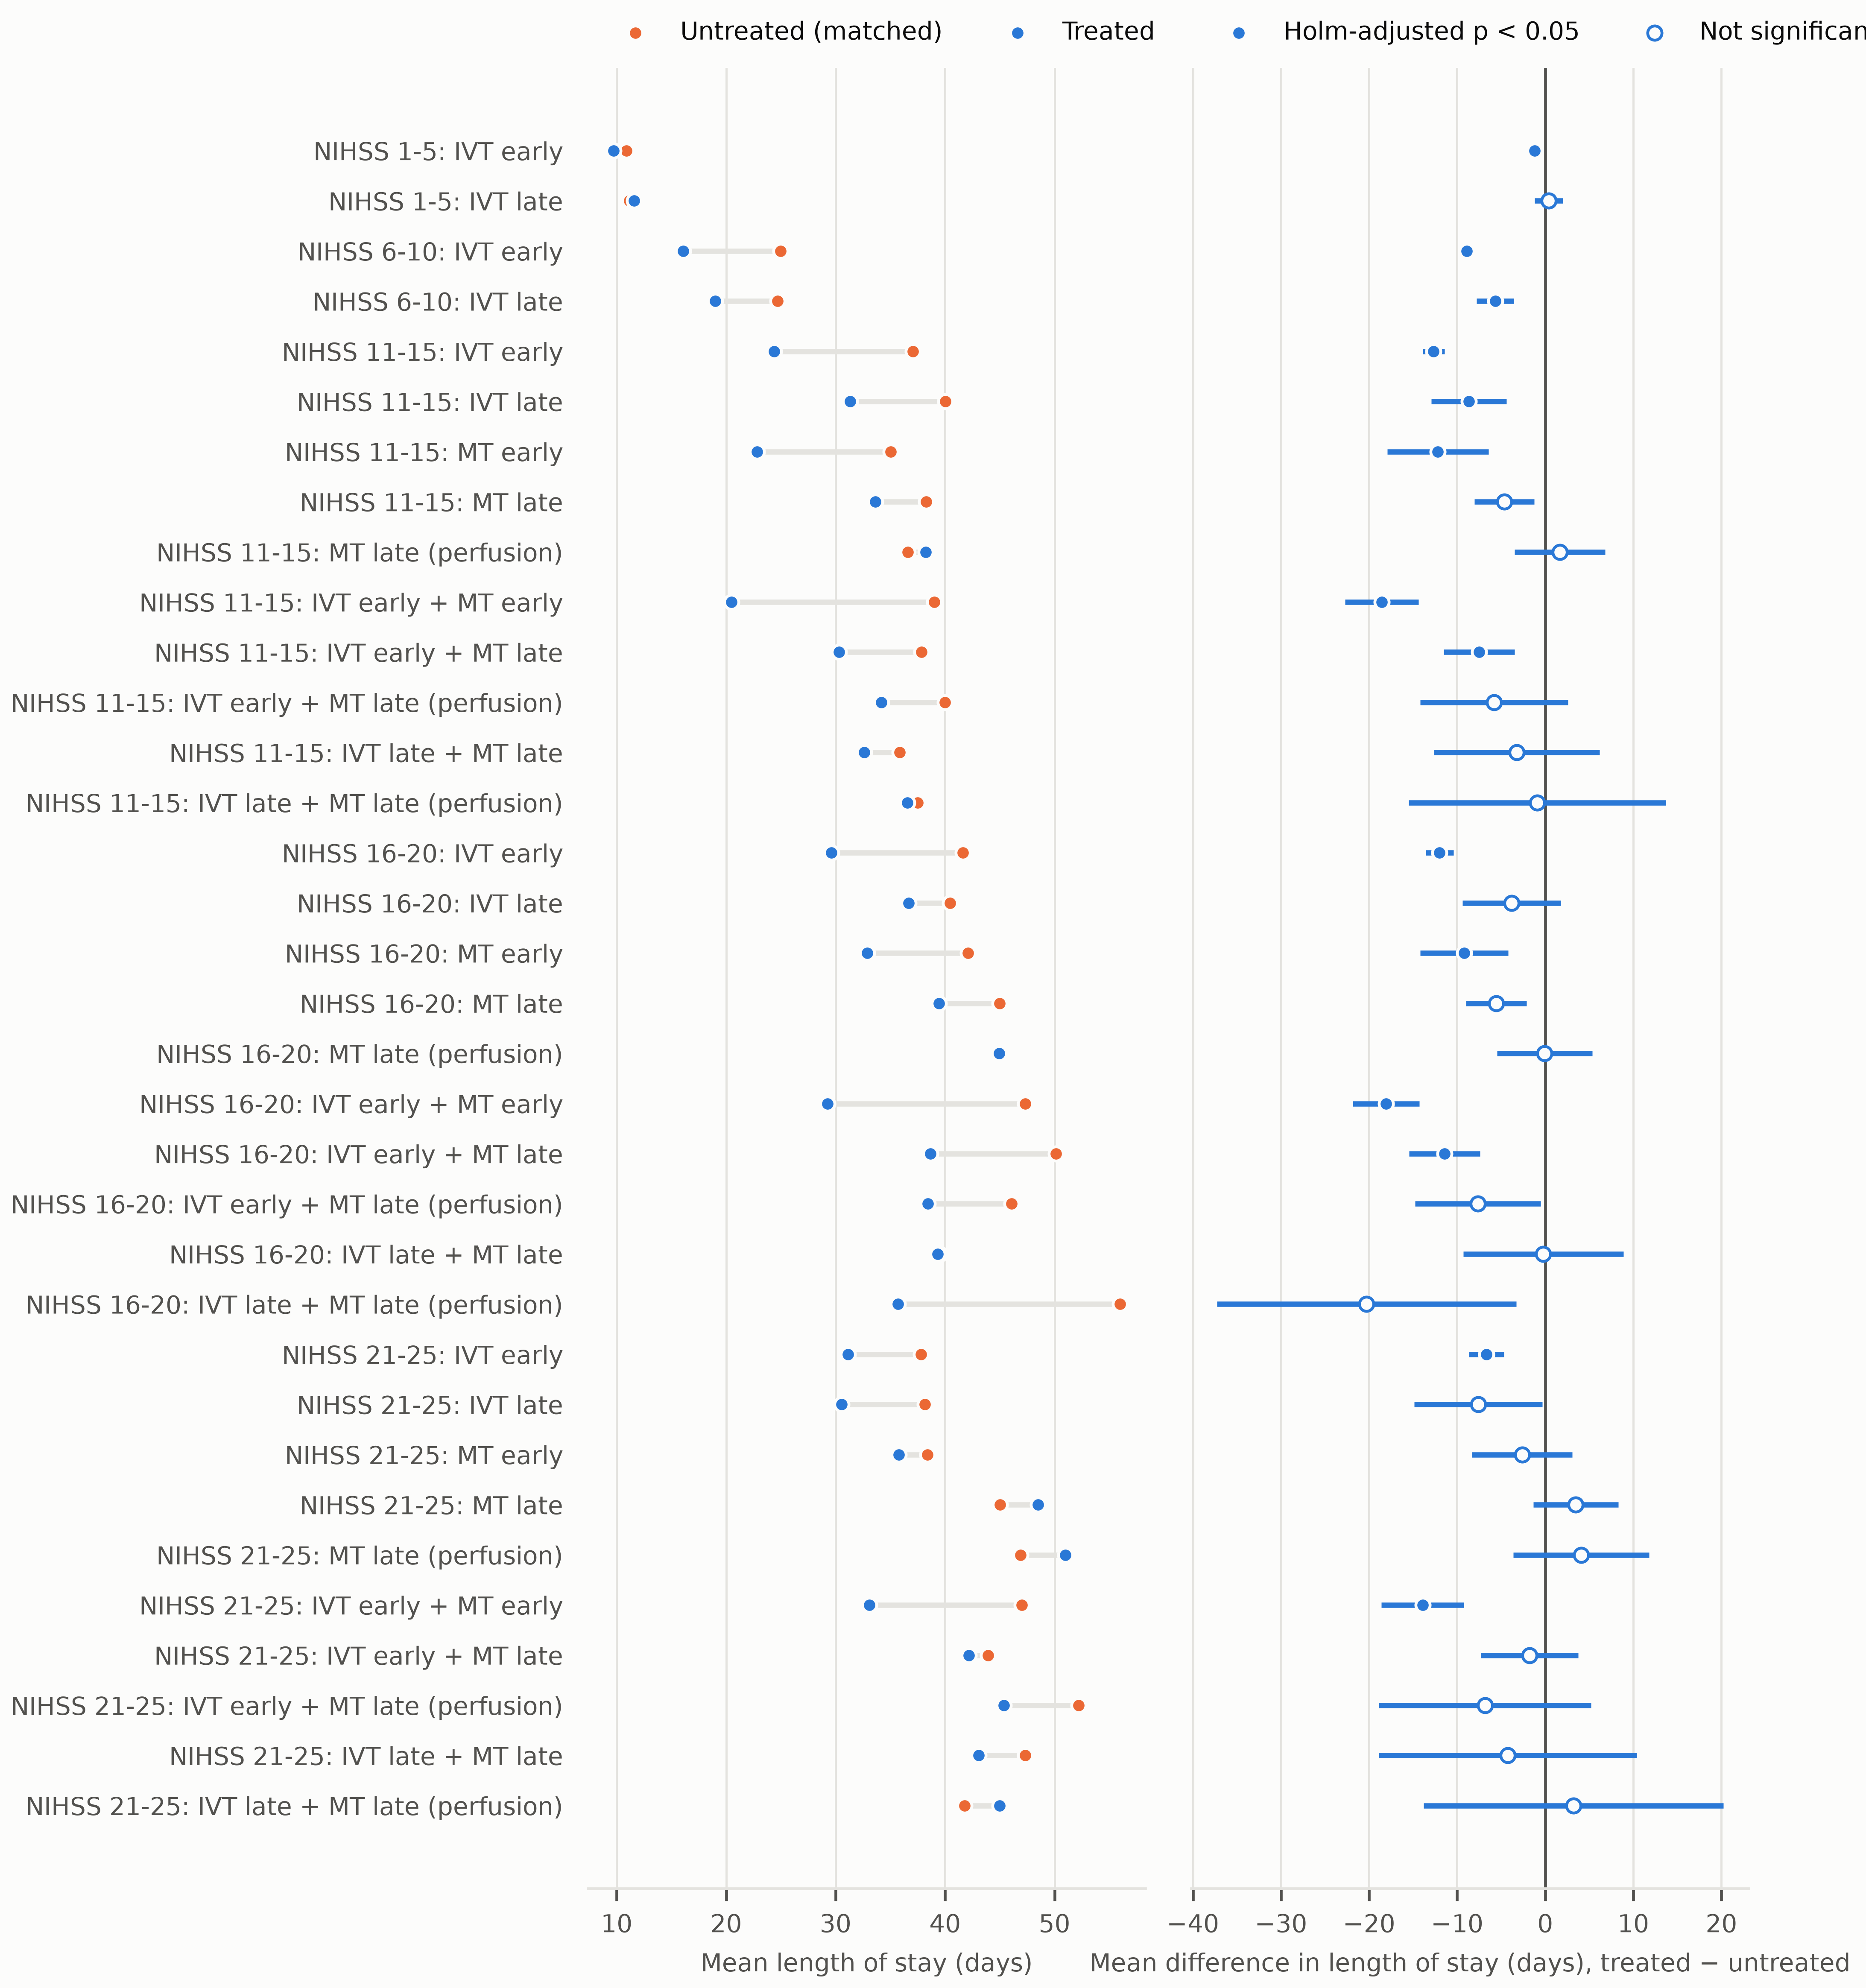
\includegraphics[width=1\linewidth]{chapters/images/all_ischaemic_stroke_target_trials_length_of_stay_chart.png}
\caption{Length of hospital stay (days) in each trial group, including patients who died in hospital. Left: mean length of stay of treated patients (blue) and matched untreated controls (orange). Right: mean within-pair difference (treated minus untreated, days) with 95\% confidence interval; filled markers show a Holm-adjusted $p < 0.05$ (Wilcoxon signed-rank test). Full results are given in Supplementary Table~\ref{tab:supp_length_of_stay}.}
\label{fig:length_of_stay}
{\small\textit{Alt text:} Two-panel dot plot for 34 trial groups ordered by stroke severity band. The left panel shows mean length of hospital stay in days for treated and matched untreated patients. The right panel shows the mean difference in days with 95\% confidence intervals. Stays are shorter with treatment in most groups, by up to about 18 days.\par}
\end{figure}

% Discharge destination

\begin{figure}
\centering
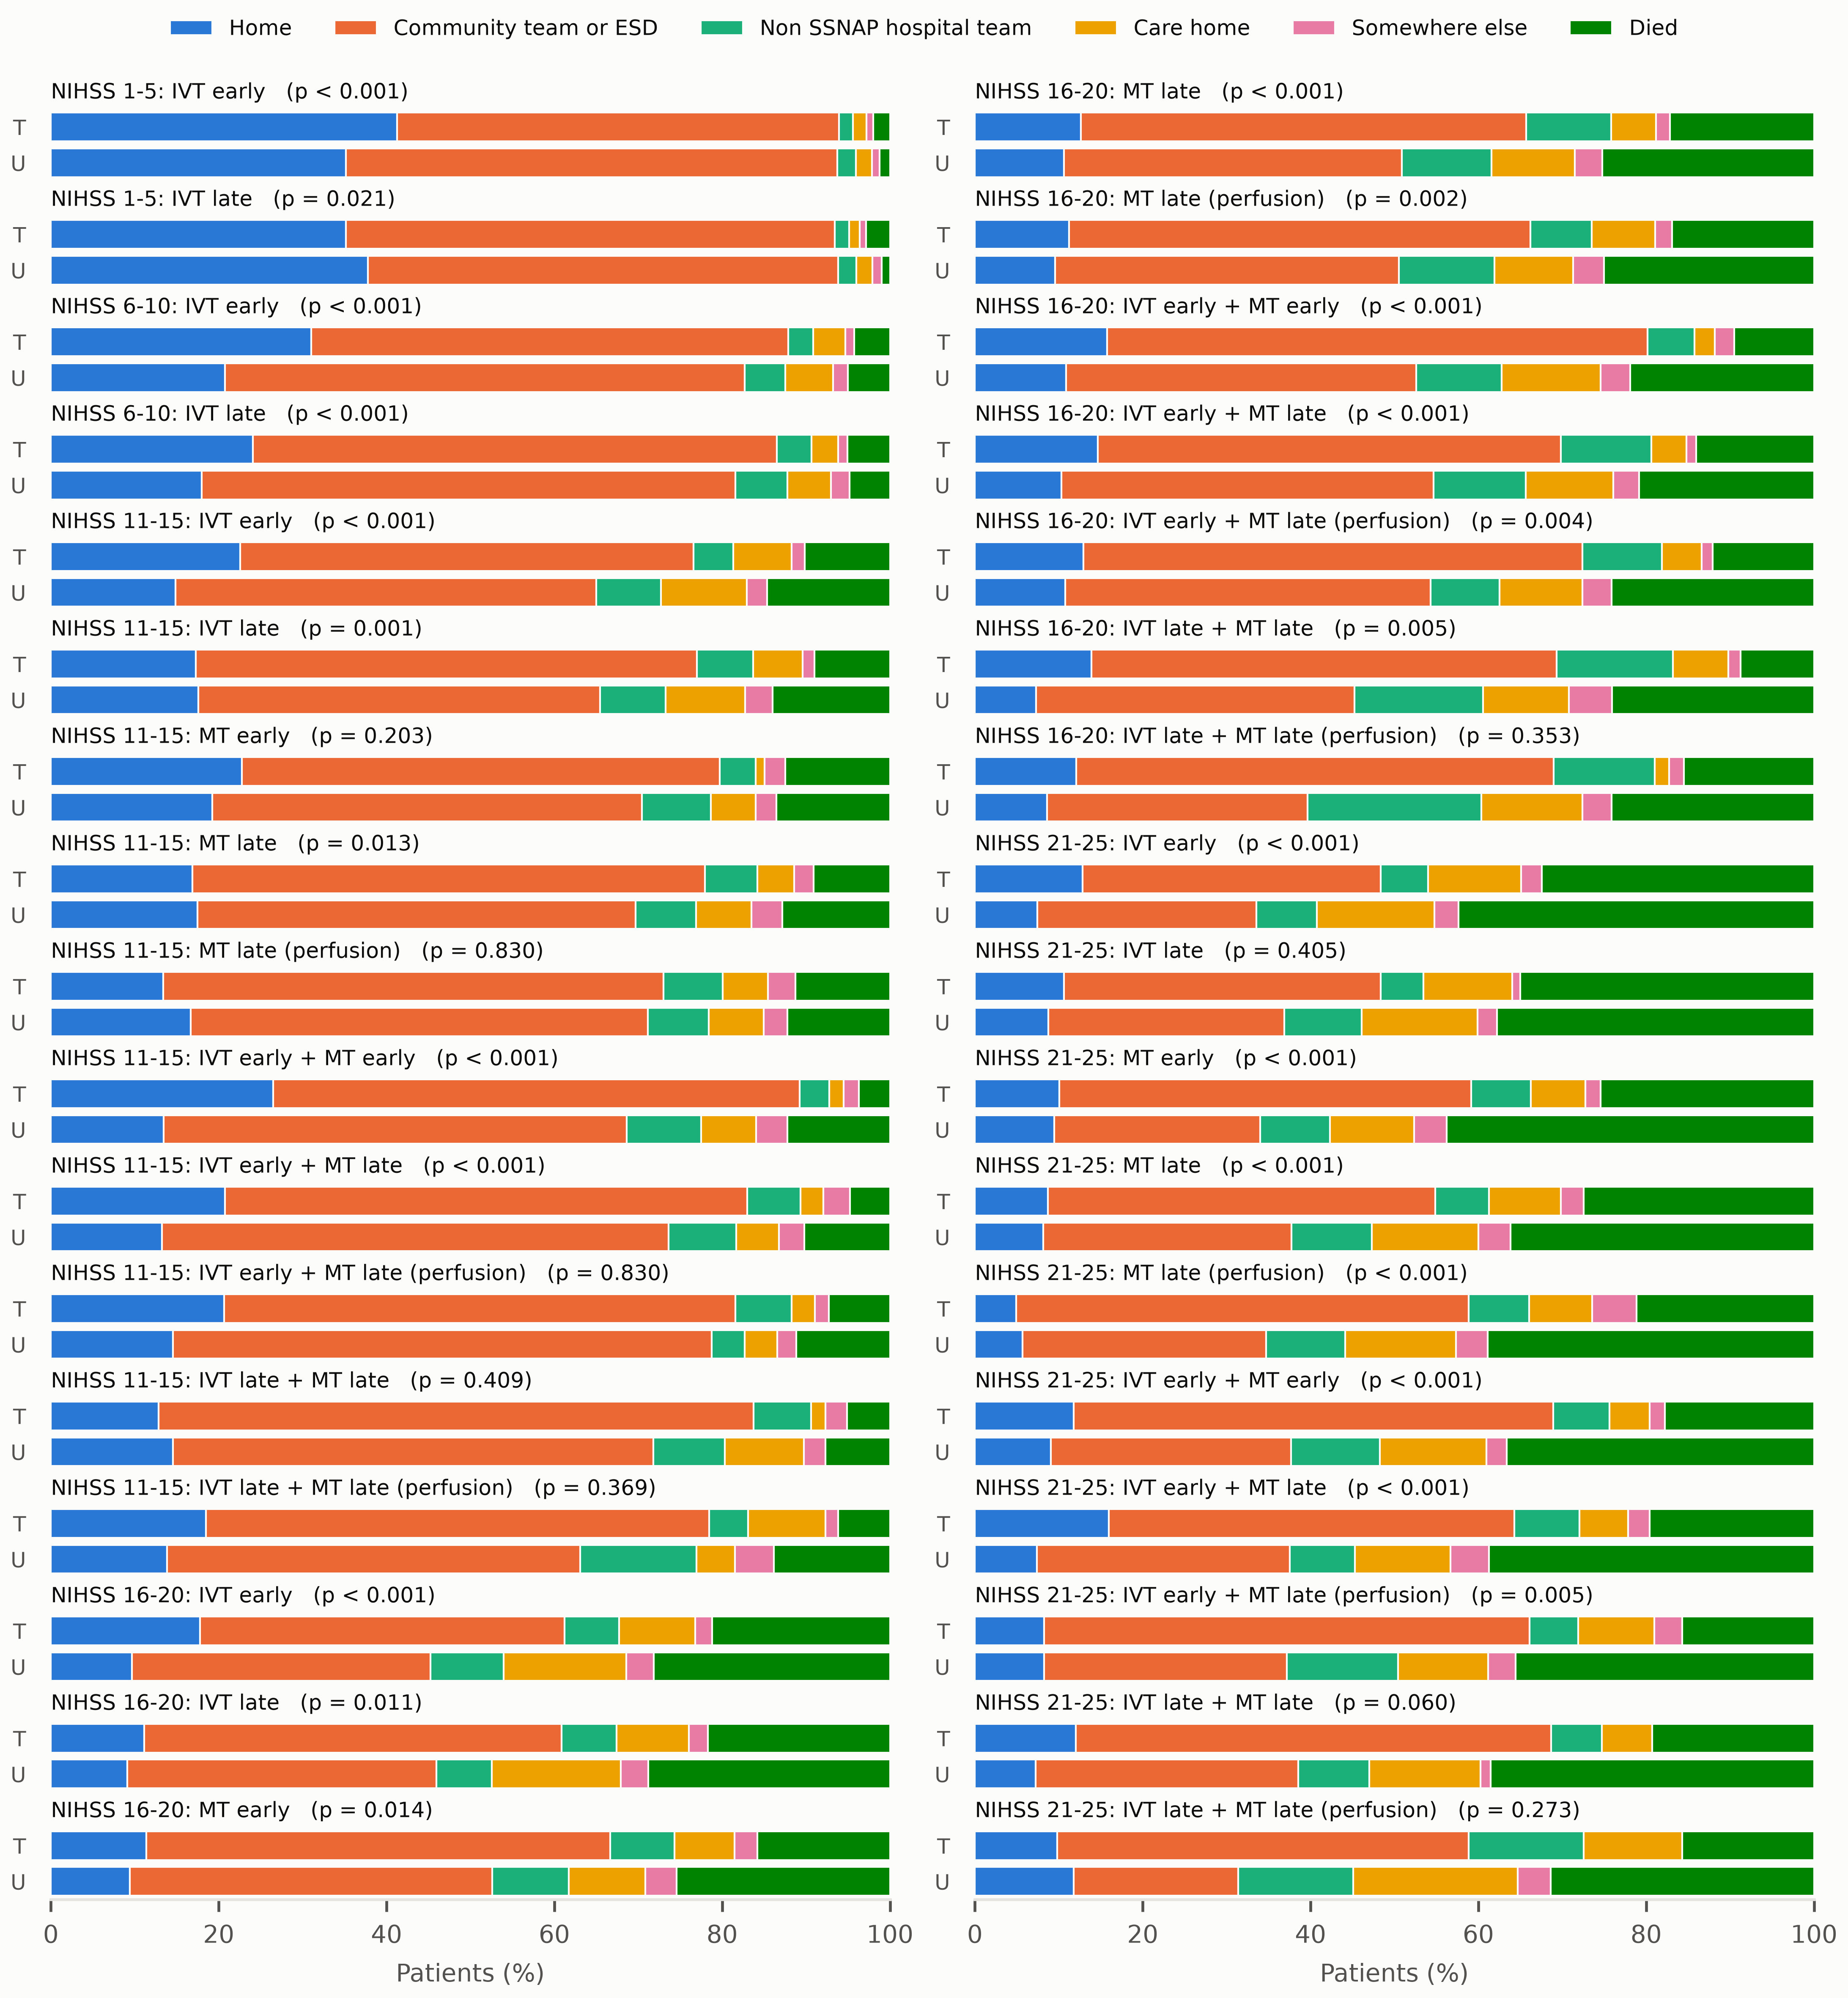
\includegraphics[width=1\linewidth,height=0.75\textheight,keepaspectratio]{chapters/images/all_ischaemic_stroke_target_trials_discharge_destination_chart.png}
\caption{Discharge destination in each trial group. Bars show the percentage of patients discharged to each destination for the treated (T) and matched untreated (U) arm of each group. The Holm-adjusted $p$-value from the Stuart--Maxwell test of marginal homogeneity is given after each group name. ESD, early supported discharge. Full results are given in Supplementary Table~\ref{tab:supp_discharge_destination}.}
\label{fig:discharge_destination}
{\small\textit{Alt text:} Horizontal stacked bar chart in two panels, with a pair of bars, treated and matched untreated, for each of 34 trial groups. Each bar shows the percentage discharged home, with community team or early supported discharge, to another hospital team, to a care home, elsewhere, or who died. Treated patients more often went home and less often went to a care home or died.\par}
\end{figure}

\section{Discussion}

\subsection{Main findings}

In this national registry study, we emulated 34 target trials of reperfusion treatment for ischaemic stroke, defined by stroke severity, type and timing of treatment, and use of perfusion imaging. Across most groups, treatment with IVT, MT or both was associated with more patients having a good outcome at discharge, lower discharge disability, fewer in-hospital deaths, shorter hospital stays and more discharges home.

We asked how these associations vary with stroke severity, with the type and timing of treatment, and across outcomes. First, they varied strongly with severity. They were small in mild stroke (NIHSS 1--5) and much larger in moderate to severe stroke. Second, they varied with treatment strategy. They were largest when IVT and MT were both given within 4.5 hours of onset, and were generally larger for early than for late treatment. Third, the pattern was broadly consistent across the five outcomes, with two exceptions: in-hospital death was slightly higher with IVT in mild stroke, and hospital stay was longer after late MT in the most severe strokes.

\subsection{Comparison with clinical trials}

The direction of our findings is consistent with trial evidence. Trials show that alteplase given within 4.5 hours improves outcome across a wide range of stroke severity\cite{emberson_effect_2014}, that thrombectomy substantially reduces disability in large-vessel occlusion\cite{goyal_endovascular_2016}, and that thrombectomy remains effective in later time windows in selected patients\cite{nogueira_thrombectomy_2018, albers_thrombectomy_2018}. We found associations in the same direction for each of these.

The size of our estimates is harder to compare with trials, and some estimates are larger than trial evidence would predict. In the pooled alteplase trials, a good outcome (mRS 0--1 at 3 to 6 months) was achieved by 32.9\% of treated patients and 23.1\% of controls when treatment was given within 3 hours, and by 35.3\% and 30.1\% when given between 3 and 4.5 hours\cite{emberson_effect_2014}. In our study, early IVT was associated with 16 to 20 percentage points more good outcomes in NIHSS 6--20. In the HERMES meta-analysis, 46.0\% of patients given thrombectomy and 26.5\% of controls were functionally independent at 90 days\cite{goyal_endovascular_2016}. Most patients in both arms also received IVT. We found differences of 23 to 34 percentage points for early IVT plus early MT, but compared with no reperfusion treatment at all, so a larger difference is expected. Our outcome definition and timing also differ from those used in trials: we measured outcome at discharge, and counted a return to pre-stroke mRS as a good outcome.

The clearest difference from trials is in mortality. Alteplase did not reduce 90-day mortality in the pooled trials (17.9\% with alteplase and 16.5\% with control)\cite{emberson_effect_2014}, and mortality did not differ significantly between arms in HERMES\cite{goyal_endovascular_2016}. In contrast, we found that in-hospital death was up to 12 percentage points lower with early IVT alone, and up to 21 percentage points lower with early IVT plus early MT. In-hospital death is not the same as 90-day mortality, but differences of this size are unlikely to be explained by treatment alone. They probably reflect, at least in part, the biases described below: patients who are dying or who are not for active treatment are less likely to receive reperfusion treatment. The mortality results in particular should therefore be interpreted with caution.

\subsection{Variation with stroke severity}

In mild stroke, the association with early IVT was small (3.0 percentage points more patients with a good outcome), and late IVT was not associated with benefit. About three quarters of untreated patients in this group had a good outcome, which leaves little room for improvement. In-hospital death was slightly higher with IVT, although deaths were rare in both arms. This is in keeping with the PRISMS trial, which found no benefit of alteplase in minor non-disabling stroke\cite{khatri_effect_2018}, and with the known risk of intracranial haemorrhage after alteplase\cite{emberson_effect_2014}. Two features of our analysis may also work against treatment in this group. Patients were matched on NIHSS band and not on exact score, and within the NIHSS 1--5 band treated patients had higher scores than their matched controls (mean 3.7 \textit{vs} 2.6 for early IVT; Supplementary Table~\ref{tab:supp_baseline_unmatched}). They are therefore likely to have had more disabling deficits. We also could not separate disabling from non-disabling deficits.

In moderate to severe stroke, treatment was associated with large differences in every outcome. The form of the association changed with severity. The difference in good outcome was generally greatest in NIHSS 11--20 and smaller in NIHSS 21--42, where a good outcome was uncommon in both arms. The differences in death and in discharge home or with community support were generally greatest in the most severe strokes.

\subsection{Variation with type and timing of treatment}

The combination of early IVT and early MT was associated with some of the largest improvements across outcomes. Within each severity band, associations were generally larger when treatment was given within 4.5 hours of onset than when it was given later or at an unknown time. This is consistent with trial evidence that the benefit of reperfusion treatment falls with time from onset\cite{emberson_effect_2014}.

These comparisons between trial groups are indirect and should be made with care. Each group was compared with its own untreated controls, and the patients who receive each treatment strategy differ. For example, between a quarter and a half of patients given MT without IVT were anticoagulated (Table~\ref{tab:baseline_matched}), which commonly rules out IVT, and patients given late MT may have been transferred from another hospital. Differences between groups may therefore reflect differences in patients as well as differences in treatment.

Associations were weaker, and often not statistically significant, in groups treated late with perfusion imaging. This should not be read as evidence that perfusion-selected treatment is ineffective. These groups were small, and patients who have perfusion imaging are likely to differ from other late-treated patients in ways we could not measure, such as unknown onset time, wake-up stroke or imaging findings. In addition, perfusion imaging is recorded in the thrombectomy section of SSNAP, so we could not identify patients selected for late IVT by perfusion imaging, as in EXTEND\cite{ma_thrombolysis_2019, campbell_extending_2019}.

\subsection{Outcomes beyond functional status}

This study reports outcomes that are rarely available from trials but matter to patients and health services. Treatment was associated with large shifts in discharge destination, with more patients going home or with community team support, and fewer going to a care home or dying in hospital. Hospital stays were generally shorter, with reductions of up to about 18 days with early IVT plus early MT. The exception was late MT in the most severe strokes, which was associated with longer stays. This group also had fewer in-hospital deaths, so the longer stay may reflect more severely affected patients surviving and needing rehabilitation. Length of stay therefore needs to be interpreted alongside mortality.

\subsection{Strengths and limitations}

The main strengths of this study are its use of national data covering most stroke admissions in England and Wales, the explicit specification of each target trial, and the reporting of several outcomes for many treatment and severity groups. Almost all treated patients were matched, so the results apply to nearly the whole treated population and not to a selected subset.

The main limitation is residual confounding. Patients were matched on a small number of variables: pre-stroke disability, NIHSS band, age band, AF diagnosis and anticoagulant use for AF. We did not adjust for other comorbidities or for process measures. Patients who were not treated may differ from treated patients in ways not captured, such as arrival time, contraindications, large-vessel occlusion, imaging findings or the reason treatment was not given. In particular, untreated controls for MT groups were not required to have a large-vessel occlusion, so their prognosis may differ from that of treated patients with the same NIHSS. Some untreated patients will not have been treated because they were judged too unwell to benefit, which would bias results in favour of treatment.

Matching on NIHSS band and not on exact score left imbalance in severity within some bands (Supplementary Table~\ref{tab:supp_baseline_unmatched}). In NIHSS 1--5, treated patients had higher scores than controls, which works against treatment. In NIHSS 21--42, treated patients had lower scores than controls in every group (mean about 24 \textit{vs} 25), which favours treatment and may explain part of the large differences seen in the most severe strokes, including in mortality. Diabetes was also less common in treated patients in most groups. Age is recorded only in 5-year bands.

Time zero was stroke onset, but treatment status was defined from treatment received at any point during the admission, and not from a decision made at onset. Patients who died or deteriorated very early, before treatment could be given, are more likely to be in the untreated group. This can make treatment look more beneficial than it is, a form of immortal time bias. Patients treated when the time of stroke onset was not known were grouped with late treatment. The late groups therefore mix treatment known to be late with treatment of unknown timing, some of which may have been given early.

Outcomes were measured at discharge and not at 90 days, as in most trials. Discharge outcomes depend on local discharge practice and the availability of rehabilitation and community services, and they may not reflect longer-term recovery. Finally, the same untreated patient could serve as a control in more than one trial group, so the groups are not independent, and many comparisons were made. We used Holm adjustment within each outcome, but small groups had limited power and wide confidence intervals.

\subsection{Implications and further work}

For clinicians and patients, these results describe what happened in routine care to patients like those who were treated, by stroke severity and treatment strategy, across outcomes that trials seldom report. They are consistent with current practice of giving reperfusion treatment as early as possible, and suggest that the expected gain from IVT in mild stroke is small. For service planners, the associations with length of stay and discharge destination are relevant to planning hospital beds, rehabilitation and community services as access to thrombectomy grows.

Further work should test how robust these estimates are. Useful analyses would include matching on exact NIHSS score, adjustment for more patient characteristics, restriction of controls for MT groups to patients with a recorded large-vessel occlusion, restriction to patients with a known onset time, and methods that handle the timing of treatment explicitly to reduce immortal time bias. Longer-term outcomes would show whether the differences seen at discharge persist.

\subsection{Conclusions}

In routine care in England and Wales, reperfusion treatment for ischaemic stroke was associated with better outcomes at discharge across most combinations of stroke severity, treatment type and timing. Associations were small in mild stroke and greatest when IVT and MT were combined early in moderate to severe stroke. By reporting death, disability, length of stay and discharge destination for each group, these results add detail that trials do not provide and that may help clinicians, patients and service planners. Because these are observational estimates that may be affected by residual confounding, they should be read as associations that complement, and do not replace, randomised evidence.


%\section{References}
\bibliographystyle{ama_esj}
%\bibliographystyle{plainnat}
%\bibliographystyle{unsrt}
%\bibliographystyle{unsrtnat}
\bibliography{references}

\section*{Acknowledgements}

We would like to thank our Patient and Carer Involvement team led by Leon Farmer (David Burgess, Simon Douglas, Ian Hancock, Nicola Hancock, John Williams), and our expert advisory group (Ajay Bhalla, Gary Ford, Martin Utley).

\section{Use of AI}

Claude (Anthropic) was used throughout this study as an assistant under the direction of the authors. It wrote Python code based on the authors' specifications; all code was run by the authors on data to which Claude had no access. It drafted and revised manuscript text, the supplementary material and the study protocol from the authors' results and instructions, and reviewed the manuscript against the TARGET reporting guideline and the journal's author guidelines. The authors made all decisions about study design, analysis and interpretation, checked all AI-generated code and text, and take full responsibility for the content of this article.

\section*{Author Contributions}

Contributions are given using the CRediT taxonomy. Conceptualisation: MA, AL, MJ, KP. Methodology: MA, AL, MJ, KP, PM, RE, MK, JD, JS, EK. Formal analysis: MA, AL, MJ, YW. Investigation: MA, AL, MJ, KP, YW, MK, JD. Software: MA, AL, KP. Validation: PM, RE, MK, JD, JS, EK, MJ, AB. Data curation: MA. Funding acquisition: MA, MJ, JS, PM, KP, AL.   Patient and public involvement: LF, LA. Writing -- original draft: MA, MJ. Writing -- review and editing: all authors.

\section*{Conflicts of interest}

None declared. 

\section*{Funding}

The authors disclose receipt of the following financial support for the research, authorship, and/or publication of this article: This research was jointly funded by the National Institute for Health and Care Research Applied Research Collaboration South West and by the National Institute for Health and Care Research Health and Social Care Delivery Research (HSDR) Programme [NIHR134326 and NIHR168927]. The funders had no role in the study design, data analysis, interpretation of the results or the decision to submit for publication.
 The views expressed in this publication are those of the authors and not necessarily those of the National Institute for Health and Care Research or the Department of Health and Social Care. 

\section*{Guarantor}

The corresponding author, Michael Allen, is the guarantor of this article.

\section*{Protocol registration}

The study protocol was not registered. A protocol, written after the analysis was completed, is given in Supplementary Section~\ref{sec:protocol}.

\section*{Data availability}

SSNAP data are available to researchers on application to the Healthcare Quality Improvement Partnership (HQIP), subject to their approval. All analysis code is archived on Zenodo (doi:10.5281/zenodo.24308374)\cite{allen_samuel3_2026} and available on GitHub (see Patients and methods).

\fi


%%%%%%%% Supplement
\ifincludesupplement

\ifincludemain
  \clearpage
\fi
\beginsupplement % Resets numbering
\centerline{{\huge Supplementary Material}}
\ifincludemain\suppcitelabels\suppnoauxcites\fi % mode 3: separate supplementary references
\section{Supplementary methods}

\section{Supplementary tables}

{\normalsize
Supplementary Table~\ref{tab:supp_baseline_unmatched} compares the matched arms on characteristics not used in matching. Supplementary Tables~\ref{tab:supp_outcome_target} to \ref{tab:supp_discharge_destination} give the full results for each emulated target trial, in the same order as the figures in the main paper. Within each table, trial groups are listed by NIHSS band and named by treatment and timing, with `(perfusion)' marking late treatment with perfusion imaging. All comparisons are between treated patients and their matched untreated controls, and Holm adjustment is across trial groups within each outcome. Trial groups with no treated patients (IVT late (perfusion) in every NIHSS band) are not shown.
\par}

% Tables generated from the target trial statistics CSV files (one per outcome).
\begin{landscape}
\footnotesize
\setlength{\tabcolsep}{4pt}

{\normalsize
Supplementary Table~\ref{tab:supp_baseline_unmatched} compares the treated and untreated arms on characteristics that were not used in matching: arrival NIHSS within the band, sex, hypertension, diabetes and congestive heart failure. The standardised mean difference (SMD, treated minus untreated) summarises the imbalance that remains after matching. Absolute values above 0.1 are often taken to indicate a meaningful imbalance.
\par}
\bigskip

\begin{longtable}{p{5.6cm}rrrrrrrrrrrrrrr}
\caption{Characteristics not used in matching in treated patients and matched untreated controls, by trial group.}\label{tab:supp_baseline_unmatched}\\
\toprule
Treatment & \multicolumn{3}{c}{Arrival NIHSS, mean} & \multicolumn{3}{c}{Male, \%} & \multicolumn{3}{c}{Hypertension, \%} & \multicolumn{3}{c}{Diabetes, \%} & \multicolumn{3}{c}{Heart failure, \%} \\
\cmidrule(lr){2-4}\cmidrule(lr){5-7}\cmidrule(lr){8-10}\cmidrule(lr){11-13}\cmidrule(lr){14-16}
 & Treated & Untreated & SMD & Treated & Untreated & SMD & Treated & Untreated & SMD & Treated & Untreated & SMD & Treated & Untreated & SMD \\
\midrule
\endfirsthead
\multicolumn{16}{l}{\textit{(continued)}}\\
\toprule
Treatment & \multicolumn{3}{c}{Arrival NIHSS, mean} & \multicolumn{3}{c}{Male, \%} & \multicolumn{3}{c}{Hypertension, \%} & \multicolumn{3}{c}{Diabetes, \%} & \multicolumn{3}{c}{Heart failure, \%} \\
\cmidrule(lr){2-4}\cmidrule(lr){5-7}\cmidrule(lr){8-10}\cmidrule(lr){11-13}\cmidrule(lr){14-16}
 & Treated & Untreated & SMD & Treated & Untreated & SMD & Treated & Untreated & SMD & Treated & Untreated & SMD & Treated & Untreated & SMD \\
\midrule
\endhead
\midrule
\multicolumn{16}{r}{\textit{Continued on next page}}\\
\endfoot
\bottomrule
\endlastfoot
\multicolumn{16}{l}{\textbf{NIHSS 1--5}}\\
IVT early & 3.7 & 2.6 & 0.83 & 61.4 & 58.8 & 0.05 & 51.2 & 54.5 & $-$0.07 & 19.0 & 24.1 & $-$0.12 & 3.5 & 3.4 & 0.01 \\
IVT late & 3.6 & 2.6 & 0.74 & 63.8 & 61.0 & 0.06 & 53.9 & 52.9 & 0.02 & 18.7 & 25.4 & $-$0.16 & 3.3 & 3.3 & 0.00 \\
\addlinespace
\multicolumn{16}{l}{\textbf{NIHSS 6--10}}\\
IVT early & 7.6 & 7.4 & 0.18 & 57.5 & 55.8 & 0.03 & 53.6 & 55.5 & $-$0.04 & 21.5 & 26.6 & $-$0.12 & 4.4 & 4.2 & 0.01 \\
IVT late & 7.6 & 7.5 & 0.09 & 58.0 & 52.8 & 0.10 & 55.7 & 56.5 & $-$0.02 & 23.6 & 27.1 & $-$0.08 & 4.3 & 4.2 & 0.01 \\
\addlinespace
\multicolumn{16}{l}{\textbf{NIHSS 11--15}}\\
IVT early & 12.8 & 12.7 & 0.03 & 53.8 & 49.8 & 0.08 & 54.4 & 55.4 & $-$0.02 & 22.3 & 24.1 & $-$0.04 & 5.0 & 5.3 & $-$0.01 \\
IVT late & 12.8 & 12.7 & 0.03 & 51.9 & 49.5 & 0.05 & 56.1 & 56.1 & 0.00 & 24.4 & 23.2 & 0.03 & 6.8 & 6.2 & 0.03 \\
MT early & 13.1 & 12.6 & 0.33 & 55.2 & 57.3 & $-$0.04 & 47.7 & 53.0 & $-$0.11 & 18.9 & 27.1 & $-$0.20 & 8.5 & 6.0 & 0.10 \\
MT late & 13.0 & 12.8 & 0.16 & 52.4 & 56.7 & $-$0.09 & 48.7 & 52.5 & $-$0.08 & 17.1 & 23.2 & $-$0.15 & 7.1 & 6.9 & 0.01 \\
MT late (perfusion) & 13.0 & 12.8 & 0.20 & 51.9 & 55.4 & $-$0.07 & 56.3 & 55.6 & 0.01 & 14.3 & 24.4 & $-$0.26 & 6.6 & 7.0 & $-$0.02 \\
IVT early + MT early & 13.2 & 12.7 & 0.33 & 52.5 & 56.9 & $-$0.09 & 42.8 & 50.5 & $-$0.16 & 10.7 & 23.0 & $-$0.33 & 3.2 & 2.4 & 0.05 \\
IVT early + MT late & 13.0 & 12.7 & 0.23 & 55.6 & 56.2 & $-$0.01 & 47.8 & 49.7 & $-$0.04 & 15.3 & 20.6 & $-$0.14 & 4.0 & 3.9 & 0.01 \\
IVT early + MT late (perfusion) & 13.1 & 12.6 & 0.36 & 58.7 & 55.9 & 0.06 & 49.2 & 52.0 & $-$0.06 & 14.0 & 20.1 & $-$0.16 & 3.4 & 6.2 & $-$0.13 \\
IVT late + MT late & 13.0 & 12.8 & 0.10 & 44.4 & 50.4 & $-$0.12 & 51.3 & 55.6 & $-$0.09 & 17.1 & 19.7 & $-$0.07 & 2.6 & 6.0 & $-$0.17 \\
IVT late + MT late (perfusion) & 13.0 & 12.9 & 0.11 & 55.4 & 50.8 & 0.09 & 52.3 & 49.2 & 0.06 & 18.5 & 15.4 & 0.08 & 10.8 & 3.1 & 0.30 \\
\addlinespace
\multicolumn{16}{l}{\textbf{NIHSS 16--20}}\\
IVT early & 17.9 & 17.9 & 0.01 & 50.0 & 45.1 & 0.10 & 56.2 & 55.9 & 0.01 & 20.0 & 22.0 & $-$0.05 & 7.1 & 6.3 & 0.03 \\
IVT late & 17.9 & 17.8 & 0.10 & 47.7 & 46.7 & 0.02 & 56.3 & 58.3 & $-$0.04 & 24.0 & 22.5 & 0.04 & 8.3 & 7.6 & 0.03 \\
MT early & 18.2 & 17.8 & 0.27 & 54.1 & 51.6 & 0.05 & 51.9 & 53.8 & $-$0.04 & 18.0 & 23.7 & $-$0.14 & 12.3 & 9.4 & 0.10 \\
MT late & 18.0 & 17.9 & 0.08 & 51.9 & 51.1 & 0.02 & 50.9 & 54.0 & $-$0.06 & 18.5 & 22.7 & $-$0.10 & 8.7 & 8.0 & 0.03 \\
MT late (perfusion) & 17.9 & 18.0 & $-$0.10 & 53.6 & 50.5 & 0.06 & 50.7 & 52.1 & $-$0.03 & 19.1 & 24.6 & $-$0.13 & 7.5 & 4.3 & 0.14 \\
IVT early + MT early & 18.1 & 17.9 & 0.10 & 59.4 & 54.6 & 0.10 & 47.3 & 49.5 & $-$0.04 & 14.5 & 19.9 & $-$0.15 & 4.3 & 4.7 & $-$0.02 \\
IVT early + MT late & 18.0 & 18.0 & 0.00 & 52.3 & 55.2 & $-$0.06 & 51.5 & 51.7 & 0.00 & 16.2 & 21.1 & $-$0.13 & 4.5 & 5.0 & $-$0.02 \\
IVT early + MT late (perfusion) & 17.9 & 18.0 & $-$0.02 & 59.0 & 51.7 & 0.15 & 47.4 & 50.0 & $-$0.05 & 14.2 & 21.6 & $-$0.19 & 5.2 & 6.9 & $-$0.07 \\
IVT late + MT late & 18.1 & 18.0 & 0.10 & 46.7 & 49.6 & $-$0.06 & 42.3 & 48.2 & $-$0.12 & 15.3 & 24.8 & $-$0.24 & 2.2 & 7.3 & $-$0.24 \\
IVT late + MT late (perfusion) & 18.2 & 18.1 & 0.07 & 56.9 & 48.3 & 0.17 & 53.5 & 43.1 & 0.21 & 12.1 & 27.6 & $-$0.39 & 6.9 & 5.2 & 0.07 \\
\addlinespace
\multicolumn{16}{l}{\textbf{NIHSS 21--42}}\\
IVT early & 24.1 & 25.1 & $-$0.29 & 43.1 & 40.8 & 0.05 & 58.6 & 55.8 & 0.06 & 21.3 & 22.1 & $-$0.02 & 7.4 & 8.2 & $-$0.03 \\
IVT late & 24.8 & 24.9 & $-$0.02 & 45.4 & 39.0 & 0.13 & 58.0 & 57.7 & 0.01 & 18.0 & 28.5 & $-$0.25 & 6.9 & 8.7 & $-$0.07 \\
MT early & 24.2 & 25.1 & $-$0.23 & 54.5 & 48.4 & 0.12 & 60.4 & 57.8 & 0.05 & 17.7 & 24.7 & $-$0.17 & 13.6 & 10.5 & 0.09 \\
MT late & 24.1 & 25.1 & $-$0.25 & 52.4 & 47.9 & 0.09 & 54.7 & 53.2 & 0.03 & 21.0 & 23.2 & $-$0.05 & 8.2 & 9.0 & $-$0.03 \\
MT late (perfusion) & 24.0 & 24.9 & $-$0.23 & 51.3 & 47.2 & 0.08 & 52.3 & 45.2 & 0.14 & 14.5 & 19.0 & $-$0.12 & 8.8 & 7.7 & 0.04 \\
IVT early + MT early & 24.0 & 24.9 & $-$0.27 & 55.8 & 52.0 & 0.08 & 50.0 & 51.9 & $-$0.04 & 15.0 & 21.6 & $-$0.17 & 5.0 & 5.9 & $-$0.04 \\
IVT early + MT late & 24.2 & 25.0 & $-$0.21 & 50.5 & 51.1 & $-$0.01 & 53.2 & 52.9 & 0.01 & 17.1 & 21.4 & $-$0.11 & 4.7 & 5.3 & $-$0.03 \\
IVT early + MT late (perfusion) & 23.8 & 25.3 & $-$0.38 & 55.6 & 51.0 & 0.09 & 53.0 & 53.0 & 0.00 & 14.6 & 21.9 & $-$0.19 & 6.6 & 5.3 & 0.06 \\
IVT late + MT late & 23.8 & 25.7 & $-$0.53 & 54.1 & 47.7 & 0.13 & 55.0 & 54.1 & 0.02 & 21.1 & 23.9 & $-$0.07 & 2.8 & 5.5 & $-$0.14 \\
IVT late + MT late (perfusion) & 23.7 & 25.3 & $-$0.43 & 46.5 & 51.7 & $-$0.10 & 50.0 & 48.3 & 0.03 & 10.3 & 22.4 & $-$0.33 & 8.6 & 6.9 & 0.06 \\
\end{longtable}
\vspace{-0.5\baselineskip}
\noindent{\scriptsize SMD, standardised mean difference (treated minus untreated, divided by the pooled standard deviation). (perfusion), late treatment with perfusion imaging.}
\clearpage

{\normalsize
Supplementary Table~\ref{tab:supp_outcome_target} gives the full results for good outcome at discharge, defined as a discharge mRS of 2 or less, or a discharge mRS no worse than before the stroke (Figure~\ref{fig:outcome_target}). For each trial group it shows the number of matched pairs, the number and percentage of patients with a good outcome in each arm, the difference between arms in percentage points, and the matched-pair odds ratio. $p$-values are from McNemar's test, before and after Holm adjustment. Positive differences and odds ratios above 1 favour treatment.
\par}
\bigskip

\begin{longtable}{p{5.6cm}rrrrrrr}
\caption{Good outcome at discharge (mRS $\le$ 2, or no worse than before the stroke) in treated patients and matched untreated controls, by trial group.}\label{tab:supp_outcome_target}\\
\toprule
Treatment & Pairs & Treated, n (\%) & Untreated, n (\%) & Difference, pp (95\% CI) & Matched OR (95\% CI) & $p$ & $p$ (Holm) \\
\midrule
\endfirsthead
\multicolumn{8}{l}{\textit{(continued)}}\\
\toprule
Treatment & Pairs & Treated, n (\%) & Untreated, n (\%) & Difference, pp (95\% CI) & Matched OR (95\% CI) & $p$ & $p$ (Holm) \\
\midrule
\endhead
\midrule
\multicolumn{8}{r}{\textit{Continued on next page}}\\
\endfoot
\bottomrule
\endlastfoot
\multicolumn{8}{l}{\textbf{NIHSS 1--5}}\\
IVT early & 12,954 & 10,034 (77.5) & 9,647 (74.5) & 3.0 (2.0 to 4.0) & 1.19 (1.12 to 1.26) & $<$0.001 & $<$0.001 \\
IVT late & 1,440 & 1,062 (73.8) & 1,106 (76.8) & $-$3.1 ($-$6.1 to $-$0.1) & 0.83 (0.70 to 1.00) & 0.052 & 0.310 \\
\addlinespace
\multicolumn{8}{l}{\textbf{NIHSS 6--10}}\\
IVT early & 13,618 & 8,632 (63.4) & 6,447 (47.3) & 16.0 (14.9 to 17.2) & 2.02 (1.92 to 2.12) & $<$0.001 & $<$0.001 \\
IVT late & 1,478 & 873 (59.1) & 677 (45.8) & 13.3 (9.7 to 16.8) & 1.72 (1.48 to 2.00) & $<$0.001 & $<$0.001 \\
\addlinespace
\multicolumn{8}{l}{\textbf{NIHSS 11--15}}\\
IVT early & 6,277 & 2,952 (47.0) & 1,705 (27.2) & 19.9 (18.3 to 21.5) & 2.51 (2.32 to 2.72) & $<$0.001 & $<$0.001 \\
IVT late & 643 & 273 (42.5) & 169 (26.3) & 16.2 (11.3 to 21.1) & 2.21 (1.71 to 2.85) & $<$0.001 & $<$0.001 \\
MT early & 281 & 138 (49.1) & 90 (32.0) & 17.1 (9.6 to 24.5) & 2.30 (1.56 to 3.38) & $<$0.001 & $<$0.001 \\
MT late & 944 & 364 (38.6) & 255 (27.0) & 11.5 (7.4 to 15.7) & 1.74 (1.42 to 2.13) & $<$0.001 & $<$0.001 \\
MT late (perfusion) & 426 & 131 (30.8) & 116 (27.2) & 3.5 ($-$2.5 to 9.6) & 1.19 (0.88 to 1.60) & 0.287 & 0.655 \\
IVT early + MT early & 596 & 357 (59.9) & 153 (25.7) & 34.2 (29.0 to 39.5) & 4.34 (3.29 to 5.74) & $<$0.001 & $<$0.001 \\
IVT early + MT late & 694 & 309 (44.5) & 190 (27.4) & 17.1 (12.2 to 22.1) & 2.16 (1.71 to 2.72) & $<$0.001 & $<$0.001 \\
IVT early + MT late (perfusion) & 179 & 71 (39.7) & 58 (32.4) & 7.3 ($-$2.9 to 17.4) & 1.35 (0.88 to 2.07) & 0.198 & 0.655 \\
IVT late + MT late & 117 & 52 (44.4) & 28 (23.9) & 20.5 (8.7 to 32.3) & 2.60 (1.43 to 4.72) & 0.002 & 0.017 \\
IVT late + MT late (perfusion) & 65 & 31 (47.7) & 22 (33.8) & 13.8 ($-$3.3 to 31.0) & 1.75 (0.86 to 3.56) & 0.164 & 0.655 \\
\addlinespace
\multicolumn{8}{l}{\textbf{NIHSS 16--20}}\\
IVT early & 4,552 & 1,456 (32.0) & 651 (14.3) & 17.7 (16.1 to 19.3) & 3.12 (2.78 to 3.51) & $<$0.001 & $<$0.001 \\
IVT late & 396 & 97 (24.5) & 63 (15.9) & 8.6 (3.4 to 13.8) & 1.85 (1.26 to 2.72) & 0.002 & 0.018 \\
MT early & 405 & 139 (34.3) & 63 (15.6) & 18.8 (13.0 to 24.5) & 2.95 (2.05 to 4.24) & $<$0.001 & $<$0.001 \\
MT late & 1,067 & 272 (25.5) & 159 (14.9) & 10.6 (7.2 to 13.9) & 1.98 (1.58 to 2.48) & $<$0.001 & $<$0.001 \\
MT late (perfusion) & 491 & 129 (26.3) & 71 (14.5) & 11.8 (7.0 to 16.6) & 2.23 (1.58 to 3.15) & $<$0.001 & $<$0.001 \\
IVT early + MT early & 913 & 392 (42.9) & 133 (14.6) & 28.4 (24.5 to 32.2) & 4.75 (3.67 to 6.16) & $<$0.001 & $<$0.001 \\
IVT early + MT late & 882 & 269 (30.5) & 111 (12.6) & 17.9 (14.1 to 21.7) & 2.98 (2.31 to 3.83) & $<$0.001 & $<$0.001 \\
IVT early + MT late (perfusion) & 232 & 75 (32.3) & 37 (15.9) & 16.4 (8.5 to 24.2) & 2.41 (1.54 to 3.77) & $<$0.001 & 0.001 \\
IVT late + MT late & 137 & 55 (40.1) & 21 (15.3) & 24.8 (15.1 to 34.5) & 4.40 (2.21 to 8.74) & $<$0.001 & $<$0.001 \\
IVT late + MT late (perfusion) & 58 & 15 (25.9) & 2 (3.4) & 22.4 (10.6 to 34.3) & 14.00 (1.84 to 106.47) & $<$0.001 & 0.011 \\
\addlinespace
\multicolumn{8}{l}{\textbf{NIHSS 21--42}}\\
IVT early & 3,919 & 840 (21.4) & 339 (8.7) & 12.8 (11.3 to 14.3) & 3.04 (2.63 to 3.51) & $<$0.001 & $<$0.001 \\
IVT late & 333 & 69 (20.7) & 25 (7.5) & 13.2 (8.3 to 18.1) & 3.93 (2.23 to 6.93) & $<$0.001 & $<$0.001 \\
MT early & 457 & 118 (25.8) & 34 (7.4) & 18.4 (13.7 to 23.1) & 4.36 (2.82 to 6.73) & $<$0.001 & $<$0.001 \\
MT late & 930 & 143 (15.4) & 70 (7.5) & 7.8 (5.1 to 10.6) & 2.40 (1.74 to 3.32) & $<$0.001 & $<$0.001 \\
MT late (perfusion) & 352 & 51 (14.5) & 35 (9.9) & 4.5 ($-$0.4 to 9.4) & 1.52 (0.96 to 2.39) & 0.089 & 0.447 \\
IVT early + MT early & 846 & 266 (31.4) & 69 (8.2) & 23.3 (19.8 to 26.8) & 5.92 (4.24 to 8.28) & $<$0.001 & $<$0.001 \\
IVT early + MT late & 677 & 137 (20.2) & 49 (7.2) & 13.0 (9.5 to 16.5) & 3.51 (2.41 to 5.12) & $<$0.001 & $<$0.001 \\
IVT early + MT late (perfusion) & 151 & 28 (18.5) & 12 (7.9) & 10.6 (3.7 to 17.5) & 3.29 (1.41 to 7.66) & 0.006 & 0.043 \\
IVT late + MT late & 109 & 24 (22.0) & 7 (6.4) & 15.6 (6.3 to 24.9) & 3.83 (1.56 to 9.41) & 0.003 & 0.024 \\
IVT late + MT late (perfusion) & 58 & 10 (17.2) & 5 (8.6) & 8.6 ($-$3.5 to 20.7) & 2.25 (0.69 to 7.31) & 0.267 & 0.655 \\
\end{longtable}
\vspace{-0.5\baselineskip}
\noindent{\scriptsize Good outcome is discharge mRS $\le$ 2 or no worse than pre-stroke mRS; higher is better. Difference is treated minus untreated, in percentage points (pp). Matched odds ratio (OR) is calculated from discordant pairs. $p$-values are from McNemar's test; Holm adjustment is across trial groups. (perfusion), late treatment with perfusion imaging. Trial groups with no treated patients (IVT late (perfusion) in every NIHSS band) are not shown.}
\clearpage

{\normalsize
Supplementary Table~\ref{tab:supp_death} gives the full results for in-hospital death (Figure~\ref{fig:death}), in the same format as Supplementary Table~\ref{tab:supp_outcome_target}. Negative differences and odds ratios below 1 indicate fewer deaths in treated patients.
\par}
\bigskip

\begin{longtable}{p{5.6cm}rrrrrrr}
\caption{In-hospital death in treated patients and matched untreated controls, by trial group.}\label{tab:supp_death}\\
\toprule
Treatment & Pairs & Treated, n (\%) & Untreated, n (\%) & Difference, pp (95\% CI) & Matched OR (95\% CI) & $p$ & $p$ (Holm) \\
\midrule
\endfirsthead
\multicolumn{8}{l}{\textit{(continued)}}\\
\toprule
Treatment & Pairs & Treated, n (\%) & Untreated, n (\%) & Difference, pp (95\% CI) & Matched OR (95\% CI) & $p$ & $p$ (Holm) \\
\midrule
\endhead
\midrule
\multicolumn{8}{r}{\textit{Continued on next page}}\\
\endfoot
\bottomrule
\endlastfoot
\multicolumn{8}{l}{\textbf{NIHSS 1--5}}\\
IVT early & 12,954 & 260 (2.0) & 160 (1.2) & 0.8 (0.5 to 1.1) & 1.65 (1.35 to 2.01) & $<$0.001 & $<$0.001 \\
IVT late & 1,440 & 41 (2.8) & 14 (1.0) & 1.9 (0.9 to 2.8) & 3.25 (1.70 to 6.21) & $<$0.001 & 0.005 \\
\addlinespace
\multicolumn{8}{l}{\textbf{NIHSS 6--10}}\\
IVT early & 13,618 & 578 (4.2) & 683 (5.0) & $-$0.8 ($-$1.3 to $-$0.3) & 0.84 (0.75 to 0.94) & 0.003 & 0.035 \\
IVT late & 1,478 & 75 (5.1) & 71 (4.8) & 0.3 ($-$1.3 to 1.8) & 1.06 (0.76 to 1.47) & 0.800 & 1.000 \\
\addlinespace
\multicolumn{8}{l}{\textbf{NIHSS 11--15}}\\
IVT early & 6,277 & 639 (10.2) & 920 (14.7) & $-$4.5 ($-$5.6 to $-$3.4) & 0.63 (0.57 to 0.71) & $<$0.001 & $<$0.001 \\
IVT late & 643 & 58 (9.0) & 90 (14.0) & $-$5.0 ($-$8.5 to $-$1.5) & 0.61 (0.43 to 0.87) & 0.007 & 0.096 \\
MT early & 281 & 35 (12.5) & 38 (13.5) & $-$1.1 ($-$6.4 to 4.3) & 0.90 (0.54 to 1.51) & 0.795 & 1.000 \\
MT late & 944 & 86 (9.1) & 121 (12.8) & $-$3.7 ($-$6.4 to $-$1.0) & 0.66 (0.49 to 0.90) & 0.010 & 0.117 \\
MT late (perfusion) & 426 & 48 (11.3) & 52 (12.2) & $-$0.9 ($-$5.4 to 3.5) & 0.92 (0.61 to 1.38) & 0.754 & 1.000 \\
IVT early + MT early & 596 & 22 (3.7) & 73 (12.2) & $-$8.6 ($-$11.5 to $-$5.6) & 0.26 (0.16 to 0.44) & $<$0.001 & $<$0.001 \\
IVT early + MT late & 694 & 33 (4.8) & 71 (10.2) & $-$5.5 ($-$8.2 to $-$2.7) & 0.43 (0.28 to 0.67) & $<$0.001 & 0.003 \\
IVT early + MT late (perfusion) & 179 & 13 (7.3) & 20 (11.2) & $-$3.9 ($-$9.8 to 2.0) & 0.61 (0.29 to 1.29) & 0.265 & 1.000 \\
IVT late + MT late & 117 & 6 (5.1) & 9 (7.7) & $-$2.6 ($-$8.6 to 3.5) & 0.62 (0.20 to 1.91) & 0.581 & 1.000 \\
IVT late + MT late (perfusion) & 65 & 4 (6.2) & 9 (13.8) & $-$7.7 ($-$18.5 to 3.1) & 0.44 (0.14 to 1.44) & 0.267 & 1.000 \\
\addlinespace
\multicolumn{8}{l}{\textbf{NIHSS 16--20}}\\
IVT early & 4,552 & 965 (21.2) & 1,281 (28.1) & $-$6.9 ($-$8.7 to $-$5.2) & 0.67 (0.61 to 0.74) & $<$0.001 & $<$0.001 \\
IVT late & 396 & 86 (21.7) & 114 (28.8) & $-$7.1 ($-$12.8 to $-$1.4) & 0.65 (0.46 to 0.93) & 0.020 & 0.197 \\
MT early & 405 & 64 (15.8) & 103 (25.4) & $-$9.6 ($-$14.9 to $-$4.3) & 0.52 (0.36 to 0.75) & $<$0.001 & 0.011 \\
MT late & 1,067 & 183 (17.2) & 269 (25.2) & $-$8.1 ($-$11.4 to $-$4.7) & 0.59 (0.47 to 0.74) & $<$0.001 & $<$0.001 \\
MT late (perfusion) & 491 & 83 (16.9) & 123 (25.1) & $-$8.1 ($-$13.1 to $-$3.2) & 0.60 (0.43 to 0.82) & 0.002 & 0.029 \\
IVT early + MT early & 913 & 87 (9.5) & 200 (21.9) & $-$12.4 ($-$15.6 to $-$9.2) & 0.35 (0.27 to 0.47) & $<$0.001 & $<$0.001 \\
IVT early + MT late & 882 & 124 (14.1) & 184 (20.9) & $-$6.8 ($-$10.3 to $-$3.3) & 0.61 (0.47 to 0.79) & $<$0.001 & 0.004 \\
IVT early + MT late (perfusion) & 232 & 28 (12.1) & 56 (24.1) & $-$12.1 ($-$18.9 to $-$5.3) & 0.42 (0.25 to 0.70) & 0.001 & 0.017 \\
IVT late + MT late & 137 & 12 (8.8) & 33 (24.1) & $-$15.3 ($-$23.7 to $-$7.0) & 0.28 (0.13 to 0.60) & 0.001 & 0.017 \\
IVT late + MT late (perfusion) & 58 & 9 (15.5) & 14 (24.1) & $-$8.6 ($-$19.7 to 2.5) & 0.38 (0.10 to 1.41) & 0.227 & 1.000 \\
\addlinespace
\multicolumn{8}{l}{\textbf{NIHSS 21--42}}\\
IVT early & 3,919 & 1,384 (35.3) & 1,857 (47.4) & $-$12.1 ($-$14.1 to $-$10.0) & 0.58 (0.52 to 0.64) & $<$0.001 & $<$0.001 \\
IVT late & 333 & 131 (39.3) & 154 (46.2) & $-$6.9 ($-$14.3 to 0.4) & 0.74 (0.54 to 1.02) & 0.079 & 0.633 \\
MT early & 457 & 115 (25.2) & 198 (43.3) & $-$18.2 ($-$23.8 to $-$12.5) & 0.39 (0.28 to 0.54) & $<$0.001 & $<$0.001 \\
MT late & 930 & 264 (28.4) & 407 (43.8) & $-$15.4 ($-$19.5 to $-$11.2) & 0.48 (0.39 to 0.59) & $<$0.001 & $<$0.001 \\
MT late (perfusion) & 352 & 77 (21.9) & 135 (38.4) & $-$16.5 ($-$22.9 to $-$10.0) & 0.43 (0.30 to 0.61) & $<$0.001 & $<$0.001 \\
IVT early + MT early & 846 & 162 (19.1) & 342 (40.4) & $-$21.3 ($-$25.3 to $-$17.2) & 0.31 (0.24 to 0.40) & $<$0.001 & $<$0.001 \\
IVT early + MT late & 677 & 148 (21.9) & 286 (42.2) & $-$20.4 ($-$25.2 to $-$15.6) & 0.37 (0.29 to 0.48) & $<$0.001 & $<$0.001 \\
IVT early + MT late (perfusion) & 151 & 26 (17.2) & 62 (41.1) & $-$23.8 ($-$33.5 to $-$14.1) & 0.28 (0.15 to 0.51) & $<$0.001 & $<$0.001 \\
IVT late + MT late & 109 & 22 (20.2) & 39 (35.8) & $-$15.6 ($-$27.9 to $-$3.3) & 0.48 (0.27 to 0.88) & 0.022 & 0.200 \\
IVT late + MT late (perfusion) & 58 & 8 (13.8) & 21 (36.2) & $-$22.4 ($-$37.7 to $-$7.1) & 0.28 (0.10 to 0.75) & 0.011 & 0.117 \\
\end{longtable}
\vspace{-0.5\baselineskip}
\noindent{\scriptsize Lower is better. Difference is treated minus untreated, in percentage points (pp). Matched odds ratio (OR) is calculated from discordant pairs. $p$-values are from McNemar's test; Holm adjustment is across trial groups. (perfusion), late treatment with perfusion imaging. Trial groups with no treated patients (IVT late (perfusion) in every NIHSS band) are not shown.}
\clearpage

{\normalsize
Supplementary Table~\ref{tab:supp_discharge_disability} gives the full results for disability at discharge, measured on the modified Rankin Scale from 0 (no symptoms) to 6 (death) (Figure~\ref{fig:discharge_disability}). For each arm it shows the mean (SD) and median [IQR] discharge mRS, followed by the mean within-pair difference with its 95\% confidence interval. Negative differences indicate less disability in treated patients. $p$-values are from the Wilcoxon signed-rank test, before and after Holm adjustment.
\par}
\bigskip

\begin{longtable}{p{5.6cm}rrrrrrrr}
\caption{Discharge disability (mRS) in treated patients and matched untreated controls, by trial group.}\label{tab:supp_discharge_disability}\\
\toprule
Treatment & Pairs & \multicolumn{2}{c}{Treated} & \multicolumn{2}{c}{Untreated} & Mean difference & \multicolumn{2}{c}{$p$} \\
\cmidrule(lr){3-4}\cmidrule(lr){5-6}\cmidrule(lr){8-9}
 & & Mean (SD) & Median [IQR] & Mean (SD) & Median [IQR] & (95\% CI) & Wilcoxon & Holm \\
\midrule
\endfirsthead
\multicolumn{9}{l}{\textit{(continued)}}\\
\toprule
Treatment & Pairs & \multicolumn{2}{c}{Treated} & \multicolumn{2}{c}{Untreated} & Mean difference & \multicolumn{2}{c}{$p$} \\
\cmidrule(lr){3-4}\cmidrule(lr){5-6}\cmidrule(lr){8-9}
 & & Mean (SD) & Median [IQR] & Mean (SD) & Median [IQR] & (95\% CI) & Wilcoxon & Holm \\
\midrule
\endhead
\midrule
\multicolumn{9}{r}{\textit{Continued on next page}}\\
\endfoot
\bottomrule
\endlastfoot
\multicolumn{9}{l}{\textbf{NIHSS 1--5}}\\
IVT early & 12,954 & 1.73 (1.37) & 2 [1--3] & 1.84 (1.32) & 2 [1--3] & $-$0.11 ($-$0.14 to $-$0.08) & $<$0.001 & $<$0.001 \\
IVT late & 1,440 & 1.83 (1.43) & 2 [1--3] & 1.79 (1.28) & 2 [1--3] & 0.04 ($-$0.05 to 0.13) & 0.574 & 1.000 \\
\addlinespace
\multicolumn{9}{l}{\textbf{NIHSS 6--10}}\\
IVT early & 13,618 & 2.29 (1.53) & 2 [1--3] & 2.77 (1.47) & 3 [2--4] & $-$0.48 ($-$0.51 to $-$0.45) & $<$0.001 & $<$0.001 \\
IVT late & 1,478 & 2.41 (1.56) & 2 [1--3] & 2.84 (1.43) & 3 [2--4] & $-$0.43 ($-$0.53 to $-$0.33) & $<$0.001 & $<$0.001 \\
\addlinespace
\multicolumn{9}{l}{\textbf{NIHSS 11--15}}\\
IVT early & 6,277 & 2.97 (1.70) & 3 [2--4] & 3.64 (1.53) & 4 [3--5] & $-$0.67 ($-$0.72 to $-$0.61) & $<$0.001 & $<$0.001 \\
IVT late & 643 & 3.06 (1.66) & 3 [2--4] & 3.64 (1.53) & 4 [3--5] & $-$0.57 ($-$0.74 to $-$0.41) & $<$0.001 & $<$0.001 \\
MT early & 281 & 2.83 (1.70) & 3 [2--4] & 3.34 (1.68) & 3 [2--4] & $-$0.51 ($-$0.77 to $-$0.25) & $<$0.001 & $<$0.001 \\
MT late & 944 & 3.06 (1.58) & 3 [2--4] & 3.40 (1.59) & 3 [2--4] & $-$0.34 ($-$0.48 to $-$0.21) & $<$0.001 & $<$0.001 \\
MT late (perfusion) & 426 & 3.39 (1.59) & 4 [2--4] & 3.39 (1.56) & 3 [2--4] & 0.00 ($-$0.21 to 0.21) & 0.695 & 1.000 \\
IVT early + MT early & 596 & 2.28 (1.53) & 2 [1--3] & 3.45 (1.56) & 4 [2--4] & $-$1.17 ($-$1.34 to $-$1.00) & $<$0.001 & $<$0.001 \\
IVT early + MT late & 694 & 2.78 (1.47) & 3 [2--4] & 3.32 (1.47) & 3 [2--4] & $-$0.55 ($-$0.70 to $-$0.39) & $<$0.001 & $<$0.001 \\
IVT early + MT late (perfusion) & 179 & 2.98 (1.64) & 3 [2--4] & 3.21 (1.58) & 3 [2--4] & $-$0.23 ($-$0.57 to 0.11) & 0.147 & 0.442 \\
IVT late + MT late & 117 & 2.85 (1.47) & 3 [2--4] & 3.41 (1.38) & 4 [3--4] & $-$0.56 ($-$0.91 to $-$0.22) & 0.002 & 0.009 \\
IVT late + MT late (perfusion) & 65 & 2.58 (1.67) & 3 [1--4] & 3.38 (1.65) & 4 [2--4] & $-$0.80 ($-$1.37 to $-$0.23) & 0.005 & 0.020 \\
\addlinespace
\multicolumn{9}{l}{\textbf{NIHSS 16--20}}\\
IVT early & 4,552 & 3.70 (1.75) & 4 [3--5] & 4.39 (1.43) & 4 [4--6] & $-$0.69 ($-$0.75 to $-$0.63) & $<$0.001 & $<$0.001 \\
IVT late & 396 & 3.87 (1.56) & 4 [3--5] & 4.38 (1.45) & 4 [4--6] & $-$0.52 ($-$0.71 to $-$0.32) & $<$0.001 & $<$0.001 \\
MT early & 405 & 3.32 (1.78) & 3 [2--5] & 4.13 (1.52) & 4 [3--6] & $-$0.81 ($-$1.03 to $-$0.59) & $<$0.001 & $<$0.001 \\
MT late & 1,067 & 3.60 (1.59) & 4 [3--5] & 4.14 (1.53) & 4 [3--6] & $-$0.54 ($-$0.67 to $-$0.41) & $<$0.001 & $<$0.001 \\
MT late (perfusion) & 491 & 3.61 (1.65) & 4 [3--5] & 4.13 (1.58) & 4 [3--5.5] & $-$0.53 ($-$0.71 to $-$0.34) & $<$0.001 & $<$0.001 \\
IVT early + MT early & 913 & 2.91 (1.65) & 3 [2--4] & 4.08 (1.48) & 4 [3--5] & $-$1.17 ($-$1.31 to $-$1.03) & $<$0.001 & $<$0.001 \\
IVT early + MT late & 882 & 3.41 (1.62) & 3.5 [2--4] & 4.12 (1.46) & 4 [3--5] & $-$0.70 ($-$0.84 to $-$0.56) & $<$0.001 & $<$0.001 \\
IVT early + MT late (perfusion) & 232 & 3.33 (1.63) & 4 [2--4] & 4.09 (1.56) & 4 [3--5] & $-$0.76 ($-$1.06 to $-$0.47) & $<$0.001 & $<$0.001 \\
IVT late + MT late & 137 & 3.17 (1.65) & 3 [2--4] & 4.09 (1.54) & 4 [3--5] & $-$0.92 ($-$1.26 to $-$0.58) & $<$0.001 & $<$0.001 \\
IVT late + MT late (perfusion) & 58 & 3.43 (1.80) & 3.5 [2.25--5] & 4.48 (1.10) & 4 [4--5] & $-$1.05 ($-$1.50 to $-$0.60) & $<$0.001 & $<$0.001 \\
\addlinespace
\multicolumn{9}{l}{\textbf{NIHSS 21--42}}\\
IVT early & 3,919 & 4.34 (1.67) & 5 [3--6] & 4.94 (1.29) & 5 [4--6] & $-$0.60 ($-$0.66 to $-$0.54) & $<$0.001 & $<$0.001 \\
IVT late & 333 & 4.43 (1.68) & 5 [3--6] & 5.00 (1.17) & 5 [4--6] & $-$0.57 ($-$0.78 to $-$0.36) & $<$0.001 & $<$0.001 \\
MT early & 457 & 3.79 (1.70) & 4 [3--6] & 4.83 (1.33) & 5 [4--6] & $-$1.04 ($-$1.23 to $-$0.84) & $<$0.001 & $<$0.001 \\
MT late & 930 & 4.20 (1.53) & 4 [3--6] & 4.81 (1.37) & 5 [4--6] & $-$0.61 ($-$0.73 to $-$0.49) & $<$0.001 & $<$0.001 \\
MT late (perfusion) & 352 & 4.06 (1.48) & 4 [3--5] & 4.60 (1.49) & 5 [4--6] & $-$0.54 ($-$0.75 to $-$0.33) & $<$0.001 & $<$0.001 \\
IVT early + MT early & 846 & 3.43 (1.76) & 3 [2--5] & 4.73 (1.38) & 5 [4--6] & $-$1.30 ($-$1.43 to $-$1.16) & $<$0.001 & $<$0.001 \\
IVT early + MT late & 677 & 3.85 (1.60) & 4 [3--5] & 4.74 (1.40) & 5 [4--6] & $-$0.89 ($-$1.04 to $-$0.74) & $<$0.001 & $<$0.001 \\
IVT early + MT late (perfusion) & 151 & 3.82 (1.51) & 4 [3--5] & 4.63 (1.44) & 5 [4--6] & $-$0.81 ($-$1.11 to $-$0.51) & $<$0.001 & $<$0.001 \\
IVT late + MT late & 109 & 3.76 (1.60) & 4 [3--5] & 4.65 (1.37) & 5 [4--6] & $-$0.89 ($-$1.27 to $-$0.51) & $<$0.001 & $<$0.001 \\
IVT late + MT late (perfusion) & 58 & 3.81 (1.67) & 4 [3--5] & 4.64 (1.40) & 5 [4--6] & $-$0.83 ($-$1.36 to $-$0.30) & 0.003 & 0.013 \\
\end{longtable}
\vspace{-0.5\baselineskip}
\noindent{\scriptsize mRS at discharge (0--6, where 6 is death); lower is better. Mean difference is treated minus untreated within matched pairs. SD, standard deviation; IQR, interquartile range. $p$-values are from the Wilcoxon signed-rank test; Holm adjustment is across trial groups. (perfusion), late treatment with perfusion imaging. Trial groups with no treated patients (IVT late (perfusion) in every NIHSS band) are not shown.}
\clearpage

{\normalsize
Supplementary Table~\ref{tab:supp_length_of_stay} gives the full results for length of hospital stay in days (Figure~\ref{fig:length_of_stay}), in the same format as Supplementary Table~\ref{tab:supp_discharge_disability}. Negative differences indicate shorter stays in treated patients. Patients who died in hospital are included, with their stay counted until death, so these results should be read alongside the results for in-hospital death in Supplementary Table~\ref{tab:supp_death}.
\par}
\bigskip

\begin{longtable}{p{5.6cm}rrrrrrrr}
\caption{Length of stay (days) in treated patients and matched untreated controls, by trial group.}\label{tab:supp_length_of_stay}\\
\toprule
Treatment & Pairs & \multicolumn{2}{c}{Treated} & \multicolumn{2}{c}{Untreated} & Mean difference & \multicolumn{2}{c}{$p$} \\
\cmidrule(lr){3-4}\cmidrule(lr){5-6}\cmidrule(lr){8-9}
 & & Mean (SD) & Median [IQR] & Mean (SD) & Median [IQR] & (95\% CI) & Wilcoxon & Holm \\
\midrule
\endfirsthead
\multicolumn{9}{l}{\textit{(continued)}}\\
\toprule
Treatment & Pairs & \multicolumn{2}{c}{Treated} & \multicolumn{2}{c}{Untreated} & Mean difference & \multicolumn{2}{c}{$p$} \\
\cmidrule(lr){3-4}\cmidrule(lr){5-6}\cmidrule(lr){8-9}
 & & Mean (SD) & Median [IQR] & Mean (SD) & Median [IQR] & (95\% CI) & Wilcoxon & Holm \\
\midrule
\endhead
\midrule
\multicolumn{9}{r}{\textit{Continued on next page}}\\
\endfoot
\bottomrule
\endlastfoot
\multicolumn{9}{l}{\textbf{NIHSS 1--5}}\\
IVT early & 12,950 & 9.7 (19.3) & 3 [2--8] & 10.9 (20.2) & 4 [2--10] & $-$1.2 ($-$1.7 to $-$0.7) & $<$0.001 & $<$0.001 \\
IVT late & 1,440 & 11.6 (23.0) & 3 [2--10] & 11.2 (20.9) & 3 [2--10] & 0.4 ($-$1.2 to 2.0) & 0.492 & 1.000 \\
\addlinespace
\multicolumn{9}{l}{\textbf{NIHSS 6--10}}\\
IVT early & 13,616 & 16.1 (26.5) & 5 [2--18] & 25.0 (31.6) & 13 [5--34] & $-$8.9 ($-$9.6 to $-$8.2) & $<$0.001 & $<$0.001 \\
IVT late & 1,478 & 19.0 (27.3) & 7 [3--24] & 24.7 (31.7) & 13 [4--33.75] & $-$5.7 ($-$7.8 to $-$3.6) & $<$0.001 & $<$0.001 \\
\addlinespace
\multicolumn{9}{l}{\textbf{NIHSS 11--15}}\\
IVT early & 6,274 & 24.4 (32.2) & 11 [4--34] & 37.1 (37.8) & 25 [9--54] & $-$12.7 ($-$13.9 to $-$11.4) & $<$0.001 & $<$0.001 \\
IVT late & 643 & 31.3 (38.4) & 17 [5--46] & 40.0 (38.7) & 28 [10--58.5] & $-$8.7 ($-$13.0 to $-$4.4) & $<$0.001 & $<$0.001 \\
MT early & 281 & 22.8 (30.0) & 10 [5--30] & 35.0 (39.5) & 21 [8--53] & $-$12.2 ($-$17.9 to $-$6.4) & $<$0.001 & $<$0.001 \\
MT late & 944 & 33.6 (37.4) & 19.5 [6--50] & 38.3 (39.3) & 25 [8--58] & $-$4.6 ($-$8.1 to $-$1.2) & 0.018 & 0.267 \\
MT late (perfusion) & 426 & 38.2 (39.7) & 26 [8--54.75] & 36.6 (41.6) & 23 [8--54.75] & 1.7 ($-$3.5 to 6.8) & 0.291 & 1.000 \\
IVT early + MT early & 596 & 20.5 (32.1) & 6 [3--22] & 39.0 (41.4) & 25.5 [8--57] & $-$18.6 ($-$22.7 to $-$14.4) & $<$0.001 & $<$0.001 \\
IVT early + MT late & 694 & 30.3 (37.5) & 15 [5--41.75] & 37.8 (39.9) & 25 [10--53] & $-$7.5 ($-$11.5 to $-$3.5) & $<$0.001 & $<$0.001 \\
IVT early + MT late (perfusion) & 179 & 34.2 (36.9) & 18 [6--56.5] & 40.0 (39.9) & 30 [7.5--61] & $-$5.8 ($-$14.2 to 2.6) & 0.120 & 1.000 \\
IVT late + MT late & 117 & 32.6 (35.6) & 16 [6--49] & 35.8 (33.7) & 27 [8--55] & $-$3.2 ($-$12.6 to 6.1) & 0.501 & 1.000 \\
IVT late + MT late (perfusion) & 65 & 36.6 (51.9) & 13 [5--58] & 37.5 (31.4) & 32 [11--55] & $-$0.9 ($-$15.5 to 13.7) & 0.430 & 1.000 \\
\addlinespace
\multicolumn{9}{l}{\textbf{NIHSS 16--20}}\\
IVT early & 4,552 & 29.6 (35.3) & 15 [5--44] & 41.6 (41.1) & 30 [10--61] & $-$12.0 ($-$13.5 to $-$10.4) & $<$0.001 & $<$0.001 \\
IVT late & 396 & 36.7 (39.0) & 24.5 [7--55] & 40.5 (40.0) & 29 [10--60] & $-$3.8 ($-$9.4 to 1.8) & 0.152 & 1.000 \\
MT early & 405 & 32.9 (34.5) & 19 [6--53] & 42.1 (38.1) & 31 [12--61] & $-$9.2 ($-$14.2 to $-$4.2) & $<$0.001 & 0.002 \\
MT late & 1,066 & 39.4 (37.6) & 30 [9--59] & 45.0 (42.8) & 35 [10--65.75] & $-$5.5 ($-$9.0 to $-$2.1) & 0.005 & 0.103 \\
MT late (perfusion) & 491 & 44.9 (42.6) & 35 [11.5--67] & 45.0 (42.9) & 37 [11--68] & $-$0.1 ($-$5.5 to 5.4) & 0.949 & 1.000 \\
IVT early + MT early & 913 & 29.3 (41.2) & 13 [4--41] & 47.3 (42.7) & 39 [11--70] & $-$18.1 ($-$21.9 to $-$14.3) & $<$0.001 & $<$0.001 \\
IVT early + MT late & 882 & 38.7 (38.5) & 25 [8--60] & 50.1 (43.8) & 42 [13--75.75] & $-$11.4 ($-$15.4 to $-$7.4) & $<$0.001 & $<$0.001 \\
IVT early + MT late (perfusion) & 232 & 38.4 (39.4) & 21 [9--57.25] & 46.1 (40.1) & 37 [13--68.25] & $-$7.7 ($-$14.8 to $-$0.5) & 0.016 & 0.254 \\
IVT late + MT late & 137 & 39.3 (43.7) & 18 [6--66] & 39.5 (40.4) & 28 [7--58] & $-$0.2 ($-$9.3 to 8.9) & 0.857 & 1.000 \\
IVT late + MT late (perfusion) & 58 & 35.7 (37.9) & 22 [8.25--50] & 56.0 (47.5) & 48.5 [17.25--83.75] & $-$20.3 ($-$37.3 to $-$3.3) & 0.025 & 0.350 \\
\addlinespace
\multicolumn{9}{l}{\textbf{NIHSS 21--42}}\\
IVT early & 3,919 & 30.4 (38.0) & 15 [5--43] & 34.5 (39.8) & 18 [6--51] & $-$4.0 ($-$5.7 to $-$2.4) & $<$0.001 & $<$0.001 \\
IVT late & 333 & 29.3 (36.0) & 13 [5--40] & 38.2 (42.8) & 19 [6--60] & $-$8.9 ($-$15.0 to $-$2.8) & 0.008 & 0.135 \\
MT early & 457 & 37.9 (42.4) & 25 [7--56] & 40.1 (47.8) & 26 [6--58] & $-$2.2 ($-$7.9 to 3.5) & 0.687 & 1.000 \\
MT late & 930 & 47.9 (44.9) & 35 [12--74] & 37.7 (43.0) & 21 [6--55.75] & 10.2 (6.2 to 14.2) & $<$0.001 & $<$0.001 \\
MT late (perfusion) & 352 & 50.8 (46.2) & 39.5 [13.75--72] & 43.3 (52.2) & 22.5 [6--65.5] & 7.4 (0.1 to 14.8) & 0.007 & 0.129 \\
IVT early + MT early & 846 & 34.6 (39.7) & 17.5 [6--54] & 44.2 (48.8) & 30 [7--66.75] & $-$9.6 ($-$13.8 to $-$5.4) & $<$0.001 & $<$0.001 \\
IVT early + MT late & 677 & 41.3 (45.9) & 28 [9--58] & 42.9 (42.2) & 32 [8--65] & $-$1.6 ($-$6.2 to 3.0) & 0.371 & 1.000 \\
IVT early + MT late (perfusion) & 151 & 46.3 (39.6) & 37 [9.5--72] & 39.1 (41.2) & 26 [6.5--55.5] & 7.2 ($-$2.4 to 16.8) & 0.090 & 1.000 \\
IVT late + MT late & 109 & 44.7 (41.2) & 34 [11--65] & 41.0 (42.7) & 28 [6--66] & 3.7 ($-$7.2 to 14.6) & 0.661 & 1.000 \\
IVT late + MT late (perfusion) & 58 & 43.1 (36.1) & 32.5 [11.5--74.5] & 52.3 (54.6) & 42 [6--74.5] & $-$9.2 ($-$25.8 to 7.4) & 0.334 & 1.000 \\
\end{longtable}
\vspace{-0.5\baselineskip}
\noindent{\scriptsize Length of stay in days, including patients who died in hospital. Mean difference is treated minus untreated within matched pairs. SD, standard deviation; IQR, interquartile range. $p$-values are from the Wilcoxon signed-rank test; Holm adjustment is across trial groups. (perfusion), late treatment with perfusion imaging. Trial groups with no treated patients (IVT late (perfusion) in every NIHSS band) are not shown.}
\clearpage

{\normalsize
Supplementary Table~\ref{tab:supp_discharge_destination} gives the full results for discharge destination (Figure~\ref{fig:discharge_destination}). For each trial group, the two rows show the percentage of treated and matched untreated patients discharged to each destination. A single $p$-value per group, from the Stuart--Maxwell test with Holm adjustment, tests whether the overall distribution of destinations differs between arms. Pairs with a missing destination for either patient are excluded.
\par}
\bigskip

\begin{longtable}{p{5.6cm}rlrrrrrrr}
\caption{Discharge destination in treated patients and matched untreated controls, by trial group.}\label{tab:supp_discharge_destination}\\
\toprule
Treatment & Pairs & Arm & \makecell{Home} & \makecell{Community team /\\ ESD} & \makecell{Non-SSNAP\\ hospital team} & \makecell{Care home} & \makecell{Somewhere else} & \makecell{Died} & $p$ (Holm) \\
\midrule
\endfirsthead
\multicolumn{10}{l}{\textit{(continued)}}\\
\toprule
Treatment & Pairs & Arm & \makecell{Home} & \makecell{Community team /\\ ESD} & \makecell{Non-SSNAP\\ hospital team} & \makecell{Care home} & \makecell{Somewhere else} & \makecell{Died} & $p$ (Holm) \\
\midrule
\endhead
\midrule
\multicolumn{10}{r}{\textit{Continued on next page}}\\
\endfoot
\bottomrule
\endlastfoot
\multicolumn{10}{l}{\textbf{NIHSS 1--5}}\\
IVT early & 12,952 & Treated & 41.3 & 52.6 & 1.7 & 1.6 & 0.8 & 2.0 & $<$0.001 \\*
 & & Untreated & 35.1 & 58.6 & 2.2 & 1.9 & 0.9 & 1.2 & \\[2pt]
IVT late & 1,440 & Treated & 35.1 & 58.3 & 1.7 & 1.2 & 0.8 & 2.8 & 0.018 \\*
 & & Untreated & 37.8 & 56.0 & 2.2 & 1.9 & 1.1 & 1.0 & \\[2pt]
\addlinespace
\multicolumn{10}{l}{\textbf{NIHSS 6--10}}\\
IVT early & 13,617 & Treated & 31.0 & 56.9 & 3.0 & 3.8 & 1.1 & 4.2 & $<$0.001 \\*
 & & Untreated & 20.7 & 62.0 & 4.8 & 5.7 & 1.7 & 5.0 & \\[2pt]
IVT late & 1,478 & Treated & 24.1 & 62.4 & 4.1 & 3.2 & 1.1 & 5.1 & $<$0.001 \\*
 & & Untreated & 18.0 & 63.6 & 6.2 & 5.2 & 2.2 & 4.8 & \\[2pt]
\addlinespace
\multicolumn{10}{l}{\textbf{NIHSS 11--15}}\\
IVT early & 6,277 & Treated & 22.5 & 54.0 & 4.7 & 6.9 & 1.6 & 10.2 & $<$0.001 \\*
 & & Untreated & 14.8 & 50.2 & 7.7 & 10.3 & 2.4 & 14.7 & \\[2pt]
IVT late & 643 & Treated & 17.3 & 59.7 & 6.7 & 5.9 & 1.4 & 9.0 & 0.001 \\*
 & & Untreated & 17.6 & 47.9 & 7.8 & 9.5 & 3.3 & 14.0 & \\[2pt]
MT early & 281 & Treated & 22.8 & 56.9 & 4.3 & 1.1 & 2.5 & 12.5 & 0.152 \\*
 & & Untreated & 19.2 & 51.2 & 8.2 & 5.3 & 2.5 & 13.5 & \\[2pt]
MT late & 944 & Treated & 16.8 & 61.1 & 6.2 & 4.3 & 2.3 & 9.1 & 0.013 \\*
 & & Untreated & 17.5 & 52.2 & 7.2 & 6.6 & 3.7 & 12.8 & \\[2pt]
MT late (perfusion) & 426 & Treated & 13.4 & 59.6 & 7.0 & 5.4 & 3.3 & 11.3 & 0.830 \\*
 & & Untreated & 16.7 & 54.5 & 7.3 & 6.6 & 2.8 & 12.2 & \\[2pt]
IVT early + MT early & 596 & Treated & 26.5 & 62.8 & 3.5 & 1.7 & 1.8 & 3.7 & $<$0.001 \\*
 & & Untreated & 13.4 & 55.2 & 8.9 & 6.5 & 3.7 & 12.2 & \\[2pt]
IVT early + MT late & 694 & Treated & 20.7 & 62.2 & 6.3 & 2.7 & 3.2 & 4.8 & $<$0.001 \\*
 & & Untreated & 13.3 & 60.4 & 8.1 & 5.0 & 3.0 & 10.2 & \\[2pt]
IVT early + MT late (perfusion) & 179 & Treated & 20.7 & 60.9 & 6.7 & 2.8 & 1.7 & 7.3 & 0.830 \\*
 & & Untreated & 14.5 & 64.2 & 3.9 & 3.9 & 2.2 & 11.2 & \\[2pt]
IVT late + MT late & 117 & Treated & 12.8 & 70.9 & 6.8 & 1.7 & 2.6 & 5.1 & 0.409 \\*
 & & Untreated & 14.5 & 57.3 & 8.5 & 9.4 & 2.6 & 7.7 & \\[2pt]
IVT late + MT late (perfusion) & 65 & Treated & 18.5 & 60.0 & 4.6 & 9.2 & 1.5 & 6.2 & 0.295 \\*
 & & Untreated & 13.8 & 49.2 & 13.8 & 4.6 & 4.6 & 13.8 & \\[2pt]
\addlinespace
\multicolumn{10}{l}{\textbf{NIHSS 16--20}}\\
IVT early & 4,552 & Treated & 17.8 & 43.4 & 6.5 & 9.1 & 2.0 & 21.2 & $<$0.001 \\*
 & & Untreated & 9.6 & 35.6 & 8.7 & 14.6 & 3.3 & 28.1 & \\[2pt]
IVT late & 396 & Treated & 11.1 & 49.7 & 6.6 & 8.6 & 2.3 & 21.7 & 0.011 \\*
 & & Untreated & 9.1 & 36.9 & 6.6 & 15.4 & 3.3 & 28.8 & \\[2pt]
MT early & 405 & Treated & 11.4 & 55.3 & 7.7 & 7.2 & 2.7 & 15.8 & 0.014 \\*
 & & Untreated & 9.4 & 43.2 & 9.1 & 9.1 & 3.7 & 25.4 & \\[2pt]
MT late & 1,067 & Treated & 12.7 & 53.0 & 10.1 & 5.3 & 1.7 & 17.2 & $<$0.001 \\*
 & & Untreated & 10.6 & 40.3 & 10.7 & 9.9 & 3.3 & 25.2 & \\[2pt]
MT late (perfusion) & 491 & Treated & 11.2 & 55.0 & 7.3 & 7.5 & 2.0 & 16.9 & 0.002 \\*
 & & Untreated & 9.6 & 40.9 & 11.4 & 9.4 & 3.7 & 25.1 & \\[2pt]
IVT early + MT early & 913 & Treated & 15.8 & 64.4 & 5.6 & 2.4 & 2.3 & 9.5 & $<$0.001 \\*
 & & Untreated & 10.8 & 41.7 & 10.2 & 11.8 & 3.5 & 21.9 & \\[2pt]
IVT early + MT late & 882 & Treated & 14.6 & 55.2 & 10.8 & 4.2 & 1.1 & 14.1 & $<$0.001 \\*
 & & Untreated & 10.3 & 44.3 & 11.0 & 10.4 & 3.1 & 20.9 & \\[2pt]
IVT early + MT late (perfusion) & 232 & Treated & 12.9 & 59.5 & 9.5 & 4.7 & 1.3 & 12.1 & 0.004 \\*
 & & Untreated & 10.8 & 43.5 & 8.2 & 9.9 & 3.4 & 24.1 & \\[2pt]
IVT late + MT late & 137 & Treated & 13.9 & 55.5 & 13.9 & 6.6 & 1.5 & 8.8 & 0.005 \\*
 & & Untreated & 7.3 & 38.0 & 15.3 & 10.2 & 5.1 & 24.1 & \\[2pt]
IVT late + MT late (perfusion) & 58 & Treated & 12.1 & 56.9 & 12.1 & 1.7 & 1.7 & 15.5 & 0.294 \\*
 & & Untreated & 8.6 & 31.0 & 20.7 & 12.1 & 3.4 & 24.1 & \\[2pt]
\addlinespace
\multicolumn{10}{l}{\textbf{NIHSS 21--42}}\\
IVT early & 3,919 & Treated & 12.2 & 33.1 & 5.4 & 11.7 & 2.3 & 35.3 & $<$0.001 \\*
 & & Untreated & 6.7 & 24.0 & 6.1 & 13.0 & 2.8 & 47.4 & \\[2pt]
IVT late & 333 & Treated & 9.3 & 35.1 & 5.1 & 9.9 & 1.2 & 39.3 & 0.014 \\*
 & & Untreated & 7.2 & 22.8 & 7.5 & 13.8 & 2.4 & 46.2 & \\[2pt]
MT early & 457 & Treated & 9.8 & 47.9 & 8.3 & 6.6 & 2.2 & 25.2 & $<$0.001 \\*
 & & Untreated & 8.3 & 23.2 & 8.3 & 12.9 & 3.9 & 43.3 & \\[2pt]
MT late & 930 & Treated & 8.2 & 45.2 & 7.3 & 8.4 & 2.6 & 28.4 & $<$0.001 \\*
 & & Untreated & 6.6 & 26.6 & 7.8 & 12.5 & 2.8 & 43.8 & \\[2pt]
MT late (perfusion) & 352 & Treated & 6.2 & 52.0 & 7.7 & 7.7 & 4.5 & 21.9 & $<$0.001 \\*
 & & Untreated & 7.1 & 26.4 & 12.2 & 10.2 & 5.7 & 38.4 & \\[2pt]
IVT early + MT early & 846 & Treated & 11.6 & 55.4 & 6.3 & 5.6 & 2.0 & 19.1 & $<$0.001 \\*
 & & Untreated & 7.7 & 26.8 & 9.3 & 12.4 & 3.3 & 40.4 & \\[2pt]
IVT early + MT late & 677 & Treated & 14.0 & 47.7 & 8.1 & 5.8 & 2.5 & 21.9 & $<$0.001 \\*
 & & Untreated & 6.1 & 28.7 & 8.1 & 11.1 & 3.8 & 42.2 & \\[2pt]
IVT early + MT late (perfusion) & 151 & Treated & 7.9 & 55.6 & 7.3 & 7.9 & 4.0 & 17.2 & $<$0.001 \\*
 & & Untreated & 6.0 & 31.8 & 11.9 & 5.3 & 4.0 & 41.1 & \\[2pt]
IVT late + MT late & 109 & Treated & 12.8 & 53.2 & 9.2 & 4.6 & 0.0 & 20.2 & 0.018 \\*
 & & Untreated & 10.1 & 30.3 & 9.2 & 11.9 & 2.8 & 35.8 & \\[2pt]
IVT late + MT late (perfusion) & 58 & Treated & 12.1 & 48.3 & 12.1 & 12.1 & 1.7 & 13.8 & 0.076 \\*
 & & Untreated & 5.2 & 24.1 & 8.6 & 20.7 & 5.2 & 36.2 & \\[2pt]
\end{longtable}
\vspace{-0.5\baselineskip}
\noindent{\scriptsize Values are percentages of patients in each arm. ESD, early supported discharge. Pairs with a missing destination for either patient are excluded. $p$-values are from the Stuart--Maxwell test of marginal homogeneity, Holm-adjusted across trial groups. (perfusion), late treatment with perfusion imaging. Trial groups with no treated patients (IVT late (perfusion) in every NIHSS band) are not shown.}
\end{landscape}


% The supplement has its own reference list
\ifincludemain
  % Mode 3: read from supplement.bbl (made by compiling supplement.tex; see latexmkrc)
  \renewcommand{\refname}{Supplementary references}
  \IfFileExists{supplement.bbl}{\input{supplement.bbl}}{\typeout{No file supplement.bbl: compile supplement.tex to make the supplementary reference list.}}
\else
  \bibliographystyle{ama_esj}
  \bibliography{references}
\fi

\fi


% Word counts - Don't count these!
%TC:ignore
%\section{Word counts}
%\detailtexcount{main}
%TC:endignore

\end{document}

